
\chapter{Cardinality}
\label{ch:card}

{\em The very existence of flame-throwers proves that some time, 
somewhere, someone said to themselves, ``You know, I want to set 
those people over there on fire, but I'm just not close enough 
to get the job done.'' --George Carlin}

\section{Equivalent sets}
\label{sec:equiv_sets}

We have seen several interesting examples of equivalence relations 
already, and in this section we will explore one more: we'll say two sets are equivalent
if they have the same number of elements. Usually, an equivalence relation
has the effect that it highlights one characteristic of the objects being studied,
while ignoring all the others. Equivalence of sets brings the issue of size (a.k.a.
cardinality) into sharp focus while, at the same time, it forgets all about the
many other features of sets. Sets that are equivalent (under the relation we
are discussing) are sometimes said to be \index{equinumerous}
\emph{equinumerous}
\footnote{Perversely, there are also those who use the term \emph{equipollent} 
to indicate that sets are the same size. This term actually applies to 
logical statements that are deducible from one another.}.

A couple of examples may be in order.

\begin{itemize}
\item If $A = \{1, 2, 3\}$ and $B = \{a, b, c\}$ then $A$ and $B$ are equivalent.
\item Since the empty set is unique -- $\emptyset$ is the only set having 0 elements -- it
follows that there are no other sets equivalent to it.
\item Every singleton set\footnote{Recall that a 
singleton set is a set having just one element.} 
is equivalent to every other singleton set.
\end{itemize}

Hopefully these examples are relatively self-evident. Unfortunately, that
very self-evidence may tend to make you think that this notion of equivalence
isn't all that interesting ---  nothing could be further from the truth! The
notion of equivalence of sets becomes really interesting when we study infinite
sets. Once we have the right definition in hand we will be able to prove
some truly amazing results. For instance, the sets $\Naturals$ and $\Rationals$ turn out to be equivalent. Since the naturals are wholly contained in the rationals this is (to say the least) counter-intuitive! Coming up with the ``right'' definition for this concept is crucial.

We could make the following:
\begin{defi}
(Well . . . not quite.) For all sets $A$ and $B$, we say $A$ and $B$ are
equivalent, and write $A \equiv B$ iff $|A| = |B|$.
\end{defi}

The problem with this definition is that it is circular. We're trying to
come up with an equivalence relation so that the equivalence classes will
represent the various cardinalities of sets (i.e. their sizes) and we 
define the relation in terms of cardinalities. We won't get anything new 
from this.

Georg Cantor was the first person to develop the modern notion of the
equivalence of sets. His early work used the notion implicitly, but when he
finally developed the concept of one-to-one correspondences in an explicit
way he was able to prove some amazing facts. The phrase ``one-to-one correspondence''
has a fairly impressive ring to it, but one can discover what it
means by just thinking carefully about what it means to count something.

Consider the solmization syllables used for the notes of the major scale
in music; they form the set $\{\mbox{do, re, mi, fa, so, la, ti}\}$. 
What are we doing when
we count this set (and presumably come up with a total of 7 notes)? We first
point at `do' while saying `one,' then point at `re' while saying `two,' 
et cetera.
In a technical sense we are creating a one-to-one correspondence between the
set containing the seven syllables and the special set $\{1, 2, 3, 4, 5, 6, 7\}$. You should notice that this one-to-one correspondence is by no means unique. For
instance we could have counted the syllables in reverse --- a descending scale,
or in some funny order -- a little melody using each note once. The fact that
there are seven syllables in the solmization of the major scale is equivalent
to saying that there exists a one-to-one correspondence between the syllables
and the special set $\{1, 2, 3, 4, 5, 6, 7\}$.  Saying ``there exists'' in this situation may seem a bit weak since in fact there are $7! = 5040$ correspondences, but ``there exists'' is what we really want here. What exactly is a one-to-one
correspondence? Well, we've actually seen such things before -- a one-to-one
correspondence is really just a bijective function between two sets. We're
finally ready to write a definition that Georg Cantor would approve of.

\begin{defi}
For all sets $A$ and $B$, we say $A$ and $B$ are equivalent, and write
$A \equiv B$ iff there exists a one-to-one (and onto) function $f$, with $\Dom{f} = A$ and $\Rng{f} = B$.
\end{defi}

Somewhat more succinctly, one can just say the sets are equivalent iff
there is a bijection between them.

We are going to ask you to prove that the above definition defines an
equivalence relation in the exercises for this section. In order to give you a
bit of a jump start on that proof we'll outline what the proof that the relation
is symmetric should look like.

\begin{quote}
To show that the relation is symmetric we must assume that $A$
and $B$ are sets with $A \equiv B$ and show that this implies that
$B \equiv A$. According to the definition above this means that we'll
need to locate a function (that is one-to-one) from $B$ to $A$. On
the other hand, since it is given that $A \equiv B$, the definition tells
us that there actually is an injective function, $f$, from $A$ to $B$.
The inverse function $f^{-1}$ would do exactly what we'd like (namely
form a map from B to A) assuming that we can show that $f^{-1}$
has the right properties. We need to know that $f^{-1}$ is a function
(remember that in general the inverse of a function is only a
relation) and that it is one-to-one. That $f^{-1}$ is a function is a
consequence of the fact that $f$ is one-to-one. That $f^{-1}$ is one-to-one
is a consequence of the fact that $f$ is a function.
\end{quote}

The above is just a sketch of a proof. In the exercise you'll need to fill
in the rest of the details as well as provide similar arguments for reflexivity
and transitivity.

For each possible finite cardinality $k$, there are many, many sets having
that cardinality, but there is one set that stands out as the most basic -- the
set of numbers from $1$ to $k$. For each cardinality $k > 0$, we use the symbol
$\Naturals_k$ to indicate this set:

\[ \Naturals_k \; = \; \{1, 2, 3, \ldots , k\}. \]

The finite cardinalities are the equivalence classes (under the relation of
set equivalence) containing the empty set and the sets $\Naturals_k$.  
Of course there
are also infinite sets!  The prototype for an infinite set would have to be
the entire set $\Naturals$.  
The long-standing tradition is to use the 
symbol \index{Aleph--naught} 
$\aleph_0$\footnote{The Hebrew letter (capital) aleph with a %
subscript zero -- usually pronounced ``aleph naught.''} 
for the cardinality 
of sets having the same size as $\Naturals$, alternatively, such sets 
are known as ``countable.''  One could make a pretty good argument that 
it is the finite sets that are actually countable!  After all it would literally take forever to count the natural numbers!  We have to presume that the 
people who instituted
this terminology meant for ``countable'' to mean ``countable, in principle''
or ``countable if you're willing to let me keep counting forever'' or maybe
``countable if you can keep counting faster and faster and are capable of
ignoring the speed of light limitations on how fast your lips can move.''  Worse
yet, the term ``countable'' has come to be used for sets whose cardinalities are
either finite \emph{or} the size of the naturals.  If we want to refer specifically to the infinite sort of countable set most mathematicians 
use the term \index{denumerable}\emph{denumerable} (although this is not universal) or \index{countably infinite} \emph{countably infinite}.  
Finally, there are sets
whose cardinalities are bigger than the naturals.   In other words, there are
sets such that no one-to-one correspondence with $\Naturals$ is possible.  
We don't mean that people have looked for one-to-one correspondences 
between such sets and $\Naturals$ and haven't been able to find them -- we literally mean that it can't be done; and it is has been proved that it can't be done! Sets having cardinalities that are this ridiculously huge are known as \index{uncountable} \emph{uncountable}. 


\clearpage

\noindent{\large \bf Exercises --- \thesection\ }

\begin{enumerate}
\item Name four sets in the equivalence class of $\{1, 2, 3\}$.

\wbitemsep

\item Prove that set equivalence is an equivalence relation.

\wbvfill

\workbookpagebreak

\item Construct a Venn diagram showing the relationships between the sets of
sets which are finite, infinite, countable, denumerable and uncountable.

\wbvfill

\item Place the sets $\Naturals$, $\Reals$, $\Rationals$, $\Integers$, $\Integers \times \Integers$, $\Complexes$, $\Naturals_{2007}$ and $\emptyset$; 
somewhere on the Venn diagram above. (Note to students (and graders): 
there are no wrong answers to this question, the point is to see what 
your intuition about these sets says at this point.)

\wbvfill

\end{enumerate}
 
%% Emacs customization
%% 
%% Local Variables: ***
%% TeX-master: "GIAM-hw.tex" ***
%% comment-column:0 ***
%% comment-start: "%% "  ***
%% comment-end:"***" ***
%% End: ***



\newpage

\section{Examples of set equivalence}
\label{sec:examp_set_eq}

There is an ancient conundrum about what happens when an irresistible force
meets an immovable object.  In a similar spirit there are sometimes heated
debates among young children concerning which super-hero will win a fight.
Can Wolverine take Batman?  What about the Incredible Hulk versus the
Thing?  Certainly Superman is at the top of the heap in this ordering.  Or is
he?  Would the man of steel even engage in a fight with a female super-hero,
say Wonder Woman?  (Remember the 1950's sensibilities of Clark Kent's
alter ego.)

To many people the current topic will seem about as sensible as the schoolyard
discussions just alluded to.  We are concerned with knowing whether
one infinite set is bigger than another, or are they the same size. There are
generally three reasons that people disdain to consider such questions.  The
first is that, like super-heros, infinite sets are just products of the imagination.
The second is that there can be no difference because ``infinite is infinite'' -- 
once you get to the size we call infinity, you can't add something to that to
get to a bigger infinity. The third is that the answers to questions like this
are not going to earn me big piles of money so ``who cares?''

Point one is actually pretty valid.  Physicists have determined that we
appear to inhabit a universe of finite scope, containing a finite number of
subatomic particles, so in reality there can be no infinite sets.  Nevertheless,
the axioms we use to study many fields in mathematics guarantee that the
objects of consideration are indeed infinite in number.  Infinity appears as a
concept even when we know it can't appear in actuality.
Point two, the ``there's only one size of infinity'' argument is wrong.  We'll
see an informal argument showing that there are at least two sizes of infinity,
and a more formal theorem that shows there is actually an infinite hierarchy
of infinities in Section~\ref{sec:cantors_thm}

Point three, ``who cares?'' is in some sense the toughest of all to deal with.
Hopefully you'll enjoy the clever arguments to come for their own intrinsic
beauty. But, if you can figure a way to make big piles of money using this
stuff that would be nice too.

Let's get started.

Which set is bigger -- the natural numbers, $\Naturals$ or the set, 
$\Enoneg$, of nonnegative even numbers?
Both are clearly infinite, so the ``infinity is infinity'' camp might be lead
to the correct conclusion through invalid reasoning.  On the other hand,
the even numbers are contained in the natural numbers so there's a pretty
compelling case for saying the evens are somehow smaller than the naturals.  
The mathematically rigorous way to show that these sets have the same
cardinality is by displaying a one-to-one correspondence.  Given an even
number how can we produce a natural to pair it with?  And, given a natural
how can we produce an even number to pair with it?
The map $f : N \longrightarrow \Enoneg$ defined by $f(x) = 2x$ 
is clearly a function,
and just about as clearly, injective\footnote{If $x$ and $y$ are 
different numbers that map to the same value, then f(x) = f(y) so
2x = 2y. But we can cancel the 2's and derive that x = y, which is a contradiction.}.  Is the map $f$ also a surjection? In other
words, is every non-negative even number the image of some natural under
$f$?  Given some non-negative even number $e$ we need to be able to come
up with an $x$ such that $f(x) = e$.   Well, since $e$ is an even number, by the
definition of ``even'' we know that there is an integer $k$ such that $e = 2k$ 
and since $e$ is either zero or positive it follows that $k$ must also be 
either $0$ or positive. It turns out that $k$ is actually the $x$ we 
are searching for. Put more
succinctly, every non-negative even number $2k$ has a preimage, $k$, under the
map $f$.  So $f$ maps $\Naturals$ surjectively onto $\Enoneg$.
Now the sets we've just considered, 

\[ \Naturals \; = \; \{0, 1, 2, 3, 4, 5, 6, \ldots \} \]

\noindent and

\[ \Enoneg \; = \; \{0, 2, 4, 6, 8, 10, 12, \ldots \} \]

\noindent both have the feature that they can be listed -- at 
least in principle. There is a first element, followed by a 
second element, followed by a third element,
et cetera, in each set. The next set we'll look at, Z, can't be listed so easily.
To list the integers we need to let the dot-dot-dots go both forward (towards
positive infinity) and backwards (towards negative infinity),

\[ \Integers \; = \; \{ \ldots , -3, -2, -1, 0, 1, 2, 3, \ldots \}. \]

\noindent To show that the integers are actually equinumerous with the natural
numbers (which is what we're about to do -- and by the way, isn't that pretty
remarkable?) we need, essentially, to figure out a way to list the integers in
a singly infinite list. Using the symbol $\pm$ we can arrange for a singly infinite
listing, and if you think about what the symbol $\pm$ means you'll probably
come up with

\[ \Integers \; = \; \{0, 1, -1, 2, -2, 3, -3, \ldots \}. \]

\noindent This singly infinite listing of the integers does the job 
we're after in a sense
-- it displays a one-to-one correspondence with $\Naturals$.  In fact 
any singly infinite listing can be thought of as displaying a one-to-one correspondence with $\Naturals$ 
-- the first entry (or should we say zeroth entry?) in the list is corresponded
with 0, the second entry is corresponded with 1, and so on.
\medskip

\begin{tabular}{ccccccccc}
\rule{32pt}{0pt} & \rule{32pt}{0pt} & \rule{32pt}{0pt} & \rule{32pt}{0pt} & \rule{32pt}{0pt} & \rule{32pt}{0pt} & \rule{32pt}{0pt} & \rule{32pt}{0pt} \\
$0$ & $1$ & $2$ & $3$ & $4$ & $5$ & $6$ & $7$ & $\ldots$ \\
$\updownarrow$ & $\updownarrow$ & $\updownarrow$ & $\updownarrow$ & $\updownarrow$ & $\updownarrow$ & $\updownarrow$ & \\
$0$ & $1$ & $-1$ & $2$ & $-2$ & $3$ & $-3$ & $4$ & $\ldots$ \\
\end{tabular}
\medskip

To make all of this precise we need to be able to explicitly give the 
one-to-one correspondence.  It isn't enough to have a picture 
of it -- we need a
formula.  Notice that the negative integers are all paired with even naturals
and the positive integers are all paired with odd naturals.  This observation
leads us to a piecewise definition for a function that gives the bijection we
seek

\[ f(x) = \left\{ \begin{array}{cl} -x/2 \rule{16pt}{0pt} & \mbox{if x is even}\\
(x + 1)/2 & \mbox{if x is odd} \end{array} \right. .\]

By the way, notice that since 0 is even it falls into the first case, and
fortunately that formula gives the ``right'' value.

\begin{exer}
The inverse function, $f^{-1}$, must also be defined piecewise, but
based on whether the input is positive or negative. Define the inverse function.
\end{exer}

The examples we've done so far have shown that the integers, 
the natural numbers and the even naturals all have the same 
cardinality. This is the first infinite cardinal number, known 
as $\aleph_0$.  In a certain sense we could view both
of the equivalences we've shown as demonstrating that 
$2 \cdot \infty = \infty$. Our next example will lend 
credence to the rule: $\infty \cdot \infty = \infty$.  
The Cartesian product of two finite sets (the set of all 
ordered pairs with entries from the sets in question) has 
cardinality equal to the product of the cardinalities of 
the sets.   What do you suppose will happen if we let the sets
be infinite?   For instance, what is the cardinality of 
$\Naturals \times \Naturals$?   Consider this:
the subset of ordered pairs that start with a 0 can be thought of as a copy
of $\Naturals$ sitting inside this Cartesian product.  In fact 
the subset of ordered pairs
starting with any particular number gives another copy of $\Naturals$ 
inside $\Naturals \times \Naturals$.  There
are infinitely many copies of $\Naturals$  sitting inside of 
$\Naturals \times \Naturals$!  This just really ought
to get us to a larger cardinality.   The surprising result that it 
\emph{doesn't} involves an idea sometimes known as 
\index{Cantor's Snake}  ``Cantor's Snake'' -- a trick that allows 
us to list the elements of $\Naturals \times \Naturals$ in a singly 
infinite list\footnote{Cantor's snake was originally created to show 
that $\Qnoneg$ and $\Naturals$ are equinumerous.
This function was introduced in the exercises for 
Section~\ref{sec:functions}.   The version we are presenting
here avoids certain complications.}.
You can visualize the set $\Naturals \times \Naturals$ as the 
points having integer coordinates
in the first quadrant (together with the origin and the positive 
$x$ and $y$ axes).
This set of points and the path through them known as Cantor's snake is
shown in Figure~\ref{fig:cantors_snake_2}.


\begin{figure}[!btp]
\begin{picture}(0,0)%
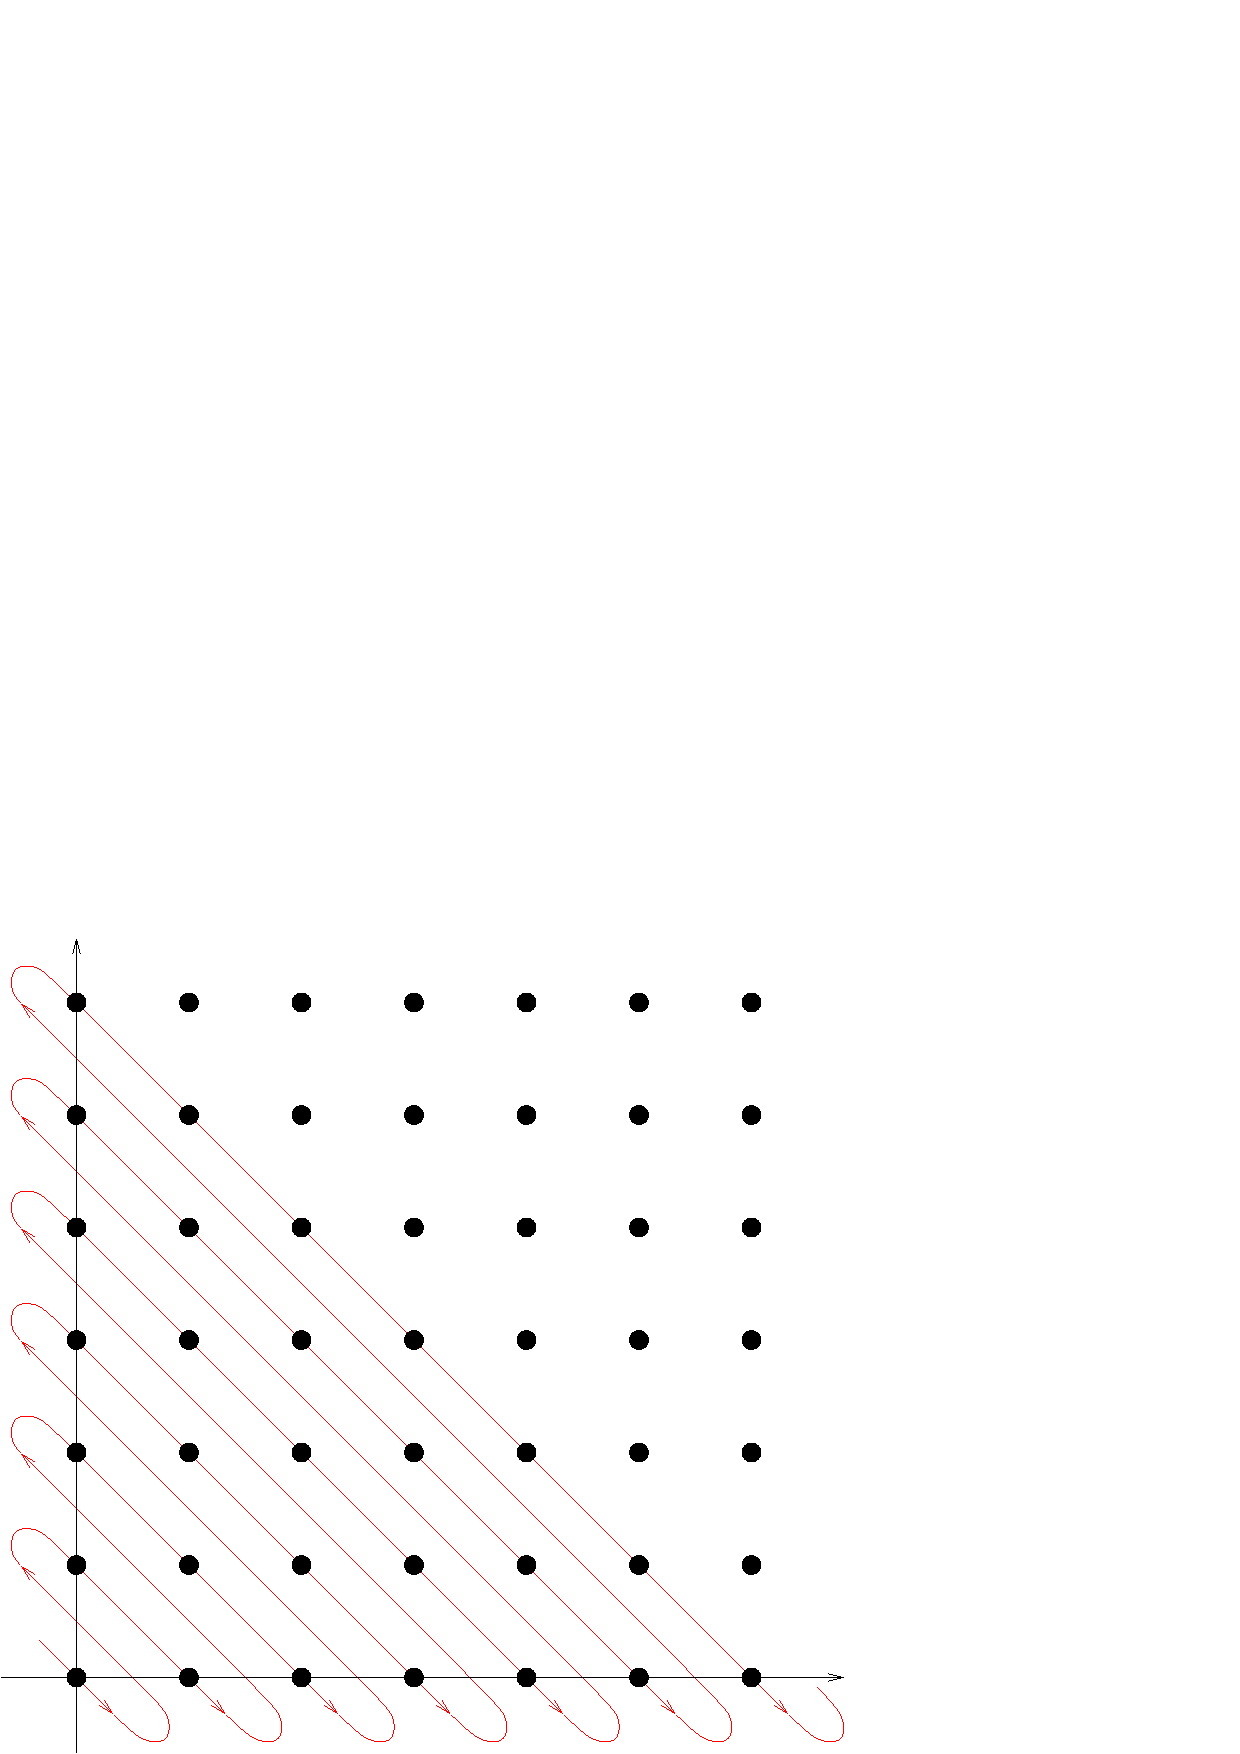
\includegraphics{figures/Cantor_snake_again.pdf}%
\end{picture}%
\setlength{\unitlength}{3947sp}%
%
\begingroup\makeatletter\ifx\SetFigFont\undefined%
\gdef\SetFigFont#1#2#3#4#5{%
  \reset@font\fontsize{#1}{#2pt}%
  \fontfamily{#3}\fontseries{#4}\fontshape{#5}%
  \selectfont}%
\fi\endgroup%
\begin{picture}(6774,6549)(589,-8173)
\put(5776,-7486){\makebox(0,0)[lb]{\smash{{\SetFigFont{12}{14.4}{\rmdefault}{\mddefault}{\updefault}{\color[rgb]{0,0,0}$(5,0)$}%
}}}}
\put(6676,-7486){\makebox(0,0)[lb]{\smash{{\SetFigFont{12}{14.4}{\rmdefault}{\mddefault}{\updefault}{\color[rgb]{0,0,0}$(6,0)$}%
}}}}
\put(1276,-7486){\makebox(0,0)[lb]{\smash{{\SetFigFont{12}{14.4}{\rmdefault}{\mddefault}{\updefault}{\color[rgb]{0,0,0}$(0,0)$}%
}}}}
\put(2176,-7486){\makebox(0,0)[lb]{\smash{{\SetFigFont{12}{14.4}{\rmdefault}{\mddefault}{\updefault}{\color[rgb]{0,0,0}$(1,0)$}%
}}}}
\put(3076,-7486){\makebox(0,0)[lb]{\smash{{\SetFigFont{12}{14.4}{\rmdefault}{\mddefault}{\updefault}{\color[rgb]{0,0,0}$(2,0)$}%
}}}}
\put(3976,-7486){\makebox(0,0)[lb]{\smash{{\SetFigFont{12}{14.4}{\rmdefault}{\mddefault}{\updefault}{\color[rgb]{0,0,0}$(3,0)$}%
}}}}
\put(4876,-7486){\makebox(0,0)[lb]{\smash{{\SetFigFont{12}{14.4}{\rmdefault}{\mddefault}{\updefault}{\color[rgb]{0,0,0}$(4,0)$}%
}}}}
\put(5776,-6586){\makebox(0,0)[lb]{\smash{{\SetFigFont{12}{14.4}{\rmdefault}{\mddefault}{\updefault}{\color[rgb]{0,0,0}$(5,1)$}%
}}}}
\put(6676,-6586){\makebox(0,0)[lb]{\smash{{\SetFigFont{12}{14.4}{\rmdefault}{\mddefault}{\updefault}{\color[rgb]{0,0,0}$(6,1)$}%
}}}}
\put(1276,-6586){\makebox(0,0)[lb]{\smash{{\SetFigFont{12}{14.4}{\rmdefault}{\mddefault}{\updefault}{\color[rgb]{0,0,0}$(0,1)$}%
}}}}
\put(2176,-6586){\makebox(0,0)[lb]{\smash{{\SetFigFont{12}{14.4}{\rmdefault}{\mddefault}{\updefault}{\color[rgb]{0,0,0}$(1,1)$}%
}}}}
\put(3076,-6586){\makebox(0,0)[lb]{\smash{{\SetFigFont{12}{14.4}{\rmdefault}{\mddefault}{\updefault}{\color[rgb]{0,0,0}$(2,1)$}%
}}}}
\put(3976,-6586){\makebox(0,0)[lb]{\smash{{\SetFigFont{12}{14.4}{\rmdefault}{\mddefault}{\updefault}{\color[rgb]{0,0,0}$(3,1)$}%
}}}}
\put(4876,-6586){\makebox(0,0)[lb]{\smash{{\SetFigFont{12}{14.4}{\rmdefault}{\mddefault}{\updefault}{\color[rgb]{0,0,0}$(4,1)$}%
}}}}
\put(5776,-5686){\makebox(0,0)[lb]{\smash{{\SetFigFont{12}{14.4}{\rmdefault}{\mddefault}{\updefault}{\color[rgb]{0,0,0}$(5,2)$}%
}}}}
\put(6676,-5686){\makebox(0,0)[lb]{\smash{{\SetFigFont{12}{14.4}{\rmdefault}{\mddefault}{\updefault}{\color[rgb]{0,0,0}$(6,2)$}%
}}}}
\put(1276,-5686){\makebox(0,0)[lb]{\smash{{\SetFigFont{12}{14.4}{\rmdefault}{\mddefault}{\updefault}{\color[rgb]{0,0,0}$(0,2)$}%
}}}}
\put(2176,-5686){\makebox(0,0)[lb]{\smash{{\SetFigFont{12}{14.4}{\rmdefault}{\mddefault}{\updefault}{\color[rgb]{0,0,0}$(1,2)$}%
}}}}
\put(3076,-5686){\makebox(0,0)[lb]{\smash{{\SetFigFont{12}{14.4}{\rmdefault}{\mddefault}{\updefault}{\color[rgb]{0,0,0}$(2,2)$}%
}}}}
\put(3976,-5686){\makebox(0,0)[lb]{\smash{{\SetFigFont{12}{14.4}{\rmdefault}{\mddefault}{\updefault}{\color[rgb]{0,0,0}$(3,2)$}%
}}}}
\put(4876,-5686){\makebox(0,0)[lb]{\smash{{\SetFigFont{12}{14.4}{\rmdefault}{\mddefault}{\updefault}{\color[rgb]{0,0,0}$(4,2)$}%
}}}}
\put(5776,-4786){\makebox(0,0)[lb]{\smash{{\SetFigFont{12}{14.4}{\rmdefault}{\mddefault}{\updefault}{\color[rgb]{0,0,0}$(5,3)$}%
}}}}
\put(6676,-4786){\makebox(0,0)[lb]{\smash{{\SetFigFont{12}{14.4}{\rmdefault}{\mddefault}{\updefault}{\color[rgb]{0,0,0}$(6,3)$}%
}}}}
\put(1276,-4786){\makebox(0,0)[lb]{\smash{{\SetFigFont{12}{14.4}{\rmdefault}{\mddefault}{\updefault}{\color[rgb]{0,0,0}$(0,3)$}%
}}}}
\put(2176,-4786){\makebox(0,0)[lb]{\smash{{\SetFigFont{12}{14.4}{\rmdefault}{\mddefault}{\updefault}{\color[rgb]{0,0,0}$(1,3)$}%
}}}}
\put(3076,-4786){\makebox(0,0)[lb]{\smash{{\SetFigFont{12}{14.4}{\rmdefault}{\mddefault}{\updefault}{\color[rgb]{0,0,0}$(2,3)$}%
}}}}
\put(3976,-4786){\makebox(0,0)[lb]{\smash{{\SetFigFont{12}{14.4}{\rmdefault}{\mddefault}{\updefault}{\color[rgb]{0,0,0}$(3,3)$}%
}}}}
\put(4876,-4786){\makebox(0,0)[lb]{\smash{{\SetFigFont{12}{14.4}{\rmdefault}{\mddefault}{\updefault}{\color[rgb]{0,0,0}$(4,3)$}%
}}}}
\put(5776,-3886){\makebox(0,0)[lb]{\smash{{\SetFigFont{12}{14.4}{\rmdefault}{\mddefault}{\updefault}{\color[rgb]{0,0,0}$(5,4)$}%
}}}}
\put(6676,-3886){\makebox(0,0)[lb]{\smash{{\SetFigFont{12}{14.4}{\rmdefault}{\mddefault}{\updefault}{\color[rgb]{0,0,0}$(6,4)$}%
}}}}
\put(1276,-3886){\makebox(0,0)[lb]{\smash{{\SetFigFont{12}{14.4}{\rmdefault}{\mddefault}{\updefault}{\color[rgb]{0,0,0}$(0,4)$}%
}}}}
\put(2176,-3886){\makebox(0,0)[lb]{\smash{{\SetFigFont{12}{14.4}{\rmdefault}{\mddefault}{\updefault}{\color[rgb]{0,0,0}$(1,4)$}%
}}}}
\put(3076,-3886){\makebox(0,0)[lb]{\smash{{\SetFigFont{12}{14.4}{\rmdefault}{\mddefault}{\updefault}{\color[rgb]{0,0,0}$(2,4)$}%
}}}}
\put(3976,-3886){\makebox(0,0)[lb]{\smash{{\SetFigFont{12}{14.4}{\rmdefault}{\mddefault}{\updefault}{\color[rgb]{0,0,0}$(3,4)$}%
}}}}
\put(4876,-3886){\makebox(0,0)[lb]{\smash{{\SetFigFont{12}{14.4}{\rmdefault}{\mddefault}{\updefault}{\color[rgb]{0,0,0}$(4,4)$}%
}}}}
\put(5776,-2986){\makebox(0,0)[lb]{\smash{{\SetFigFont{12}{14.4}{\rmdefault}{\mddefault}{\updefault}{\color[rgb]{0,0,0}$(5,5)$}%
}}}}
\put(6676,-2986){\makebox(0,0)[lb]{\smash{{\SetFigFont{12}{14.4}{\rmdefault}{\mddefault}{\updefault}{\color[rgb]{0,0,0}$(6,5)$}%
}}}}
\put(1276,-2986){\makebox(0,0)[lb]{\smash{{\SetFigFont{12}{14.4}{\rmdefault}{\mddefault}{\updefault}{\color[rgb]{0,0,0}$(0,5)$}%
}}}}
\put(2176,-2986){\makebox(0,0)[lb]{\smash{{\SetFigFont{12}{14.4}{\rmdefault}{\mddefault}{\updefault}{\color[rgb]{0,0,0}$(1,5)$}%
}}}}
\put(3076,-2986){\makebox(0,0)[lb]{\smash{{\SetFigFont{12}{14.4}{\rmdefault}{\mddefault}{\updefault}{\color[rgb]{0,0,0}$(2,5)$}%
}}}}
\put(3976,-2986){\makebox(0,0)[lb]{\smash{{\SetFigFont{12}{14.4}{\rmdefault}{\mddefault}{\updefault}{\color[rgb]{0,0,0}$(3,5)$}%
}}}}
\put(4876,-2986){\makebox(0,0)[lb]{\smash{{\SetFigFont{12}{14.4}{\rmdefault}{\mddefault}{\updefault}{\color[rgb]{0,0,0}$(4,5)$}%
}}}}
\put(5776,-2086){\makebox(0,0)[lb]{\smash{{\SetFigFont{12}{14.4}{\rmdefault}{\mddefault}{\updefault}{\color[rgb]{0,0,0}$(5,6)$}%
}}}}
\put(6676,-2086){\makebox(0,0)[lb]{\smash{{\SetFigFont{12}{14.4}{\rmdefault}{\mddefault}{\updefault}{\color[rgb]{0,0,0}$(6,6)$}%
}}}}
\put(1276,-2086){\makebox(0,0)[lb]{\smash{{\SetFigFont{12}{14.4}{\rmdefault}{\mddefault}{\updefault}{\color[rgb]{0,0,0}$(0,6)$}%
}}}}
\put(2176,-2086){\makebox(0,0)[lb]{\smash{{\SetFigFont{12}{14.4}{\rmdefault}{\mddefault}{\updefault}{\color[rgb]{0,0,0}$(1,6)$}%
}}}}
\put(3076,-2086){\makebox(0,0)[lb]{\smash{{\SetFigFont{12}{14.4}{\rmdefault}{\mddefault}{\updefault}{\color[rgb]{0,0,0}$(2,6)$}%
}}}}
\put(3976,-2086){\makebox(0,0)[lb]{\smash{{\SetFigFont{12}{14.4}{\rmdefault}{\mddefault}{\updefault}{\color[rgb]{0,0,0}$(3,6)$}%
}}}}
\put(4876,-2086){\makebox(0,0)[lb]{\smash{{\SetFigFont{12}{14.4}{\rmdefault}{\mddefault}{\updefault}{\color[rgb]{0,0,0}$(4,6)$}%
}}}}
\end{picture}%

\caption[Cantor's snake.]{Cantor's snake winds through the set %
$\Naturals \times \Naturals$ encountering its
elements one after the other.}
\label{fig:cantors_snake_2} 
\end{figure}

The diagram in Figure~\ref{fig:cantors_snake_2} gives a visual form of the one-to-one correspondence
we seek. In tabular form we would have something like the following.
\medskip

\begin{tabular}{cccccccccc}
\rule{32pt}{0pt} & \rule{32pt}{0pt} & \rule{32pt}{0pt} & \rule{32pt}{0pt} & \rule{32pt}{0pt} & \rule{32pt}{0pt} & \rule{32pt}{0pt} & \rule{32pt}{0pt} \\
$0$ & $1$ & $2$ & $3$ & $4$ & $5$ & $6$ & $7$ & $8$ & $\ldots$ \\
$\updownarrow$ & $\updownarrow$ & $\updownarrow$ & $\updownarrow$ & $\updownarrow$ & $\updownarrow$ &  $\updownarrow$ & $\updownarrow$ & $\updownarrow$ & \\
$(0, 0)$ & $(0, 1)$ & $(1, 0)$ & $(0, 2)$ & $(1, 1)$ & $(2, 0)$ & $(0, 3)$ & $(1,2)$ & $(2, 1)$ & $\ldots$ \\
\end{tabular}
\medskip

We need to produce a formula. In truth, we should really produce two
formulas.  One that takes an ordered pair $(x, y)$ and produces a number $n$.
Another that takes a number $n$ and produces an ordered pair $(x, y)$ The
number $n$ tells us where the pair $(x, y)$ lies in our infinite listing.  
There is a
problem though: the second formula (that gives the map from $\Naturals$  
to $\Naturals \times \Naturals$)
is really hard to write down -- it's easier to describe the map 
algorithmically. 
 A simple observation will help us to deduce the various formulas.  The
ordered pairs along the $y$-axis (those of the form (0, something)) correspond
to triangular numbers.  In fact the pair $(0, n)$ will correspond to the $n$-th triangular
number, $T(n) = (n^2 + n)/2$.  The ordered pairs along the descending
slanted line starting from $(0, n)$  all have the feature that the sum of their
coordinates is $n$ (because as the $x$-coordinate is increasing, the 
$y$-coordinate
is decreasing).  So, given an ordered pair $(x, y)$, the number corresponding
to the position at the upper end of the slanted line it is on (which will have
coordinates $(0, x+y)$) will be $T(x+y)$, and the pair $(x, y)$ occurs in the listing exactly $x$ positions after $(0, x + y)$.  Thus, the function 
$f : \Naturals \times \Naturals \longrightarrow N$ is
given by

\[ f(x, y) \; = \; x + T(x + y) = x + \frac{(x + y)^2 + (x + y)}{2}. \]

\noindent To go the other direction -- that is, to take a position 
in the listing and
derive an ordered pair -- we need to figure out where a given number lies
relative to the triangular numbers.  For instance, try to figure out what
$(x, y)$ pair position number $13$ will correspond with.  Well, the next smaller
triangular number is $10$ which is $T(4)$, so $13$ will be the number of an 
ordered pair along the descending line whose $y$-intercept is $4$.  
In fact, $13$ will be paired
with an ordered pair having a $3$ in the $x$-coordinate (since $13$ is $3$ 
larger than $10$) so it follows that $f^{-1}(13) = (3, 1)$.

Of course we need to generalize this procedure.  One of the hardest parts
of finding that generalization is finding the number $4$ in the above example
(when we just happen to notice that $T(4)=10$ ).  What we're really doing
there is inverting the function $T(n)$.  Finding an inverse for 
$T(n) = (n^2+n)/2$ was the essence of one of the exercises in 
Section~\ref{sec:special_functions}.  
The parabola $y = (x^2 + x)/2$ has roots at $0$ and $-1$ and is scaled by a
factor of $1/2$ relative to the ``standard'' parabola $y = x^2$.  
Its vertex is at
$(-1/2,-1/8)$.  The graph of the inverse relation is, of course, obtained by
reflecting through the line $y = x$ and by considering scaling and horizontal/
vertical translations we can deduce a formula for a function that gives a
right inverse for $T$, 

\[ T^{-1}(x) = \sqrt{2x + 1/4} - 1/2. \]

So, given $n$, a position in the listing, we calculate $A = \lfloor \sqrt{2n + 1/4}-1/2 \rfloor$.  The $x$-coordinate of our ordered pair is $n-T(A)$ 
and the $y$-coordinate is $A-x$.  
It is not pretty, but the above discussion can be translated into a formula
for $f^{-1}$.

\begin{gather*}
f^{-1}(n) \; = \; \left( n - \frac{ \lfloor \sqrt{2n + 1/4} - 1/2 \rfloor^2 + \lfloor \sqrt{2n + 1/4} - 1/2 \rfloor}{2} , \right. \\
\left. \lfloor \sqrt{2n + 1/4} - 1/2  \rfloor - n + \frac{\lfloor \sqrt{2n + 1/4} - 1/2 \rfloor^2 + \lfloor \sqrt{2n + 1/4} - 1/2 \rfloor}{2} \right).
\end{gather*}

When restricted to the appropriate sets ($f$'s domain 
is restricted to $\Naturals \times \Naturals$
and $f^{-1}$'s domain is restricted to $\Naturals$), 
these functions are two-sided inverses
for one another. That fact is sufficient to prove that $f$ 
is bijective.  
So far we have shown that the sets $\Enoneg$, $\Naturals$, $\Integers$ and 
$\Naturals \times \Naturals$ all have
the same cardinality ---  $\aleph_0$.  We plan to provide an argument that there
actually are other infinite cardinals in the next section. Before leaving the
present topic (examples of set equivalence) we'd like to present another nice
technique for deriving the bijective correspondences we use to show that sets
are equivalent -- geometric constructions.
Consider the set of points on the line segment $[0, 1]$. 
Now consider the set
of points on the line segment $[0, 2]$. This second line 
segment, being twice as
long as the first, must have a lot more points on it. Right?

Well, perhaps you're getting used to this sort of thing\ldots   
The interval $[0, 1]$ is a subset of the interval $[0, 2]$, 
but since both represent infinite sets of points
it's possible they actually have the same cardinality.  
We can prove that this is so using a geometric technique. 
We position the line segments appropriately
and then use projection from a carefully chosen point to 
develop a bijection.  Imagine both intervals as lying on 
the $x$-axis in the $x$-$y$ plane. Shift the
smaller interval up one unit so that it lies on the line 
$y = 1$.  Now, use projection
from the point $(0, 2)$, to visualize the correspondence 
see Figure~\ref{fig:equiv_intervals}

\begin{figure}[!hbtp]
\begin{picture}(0,0)%
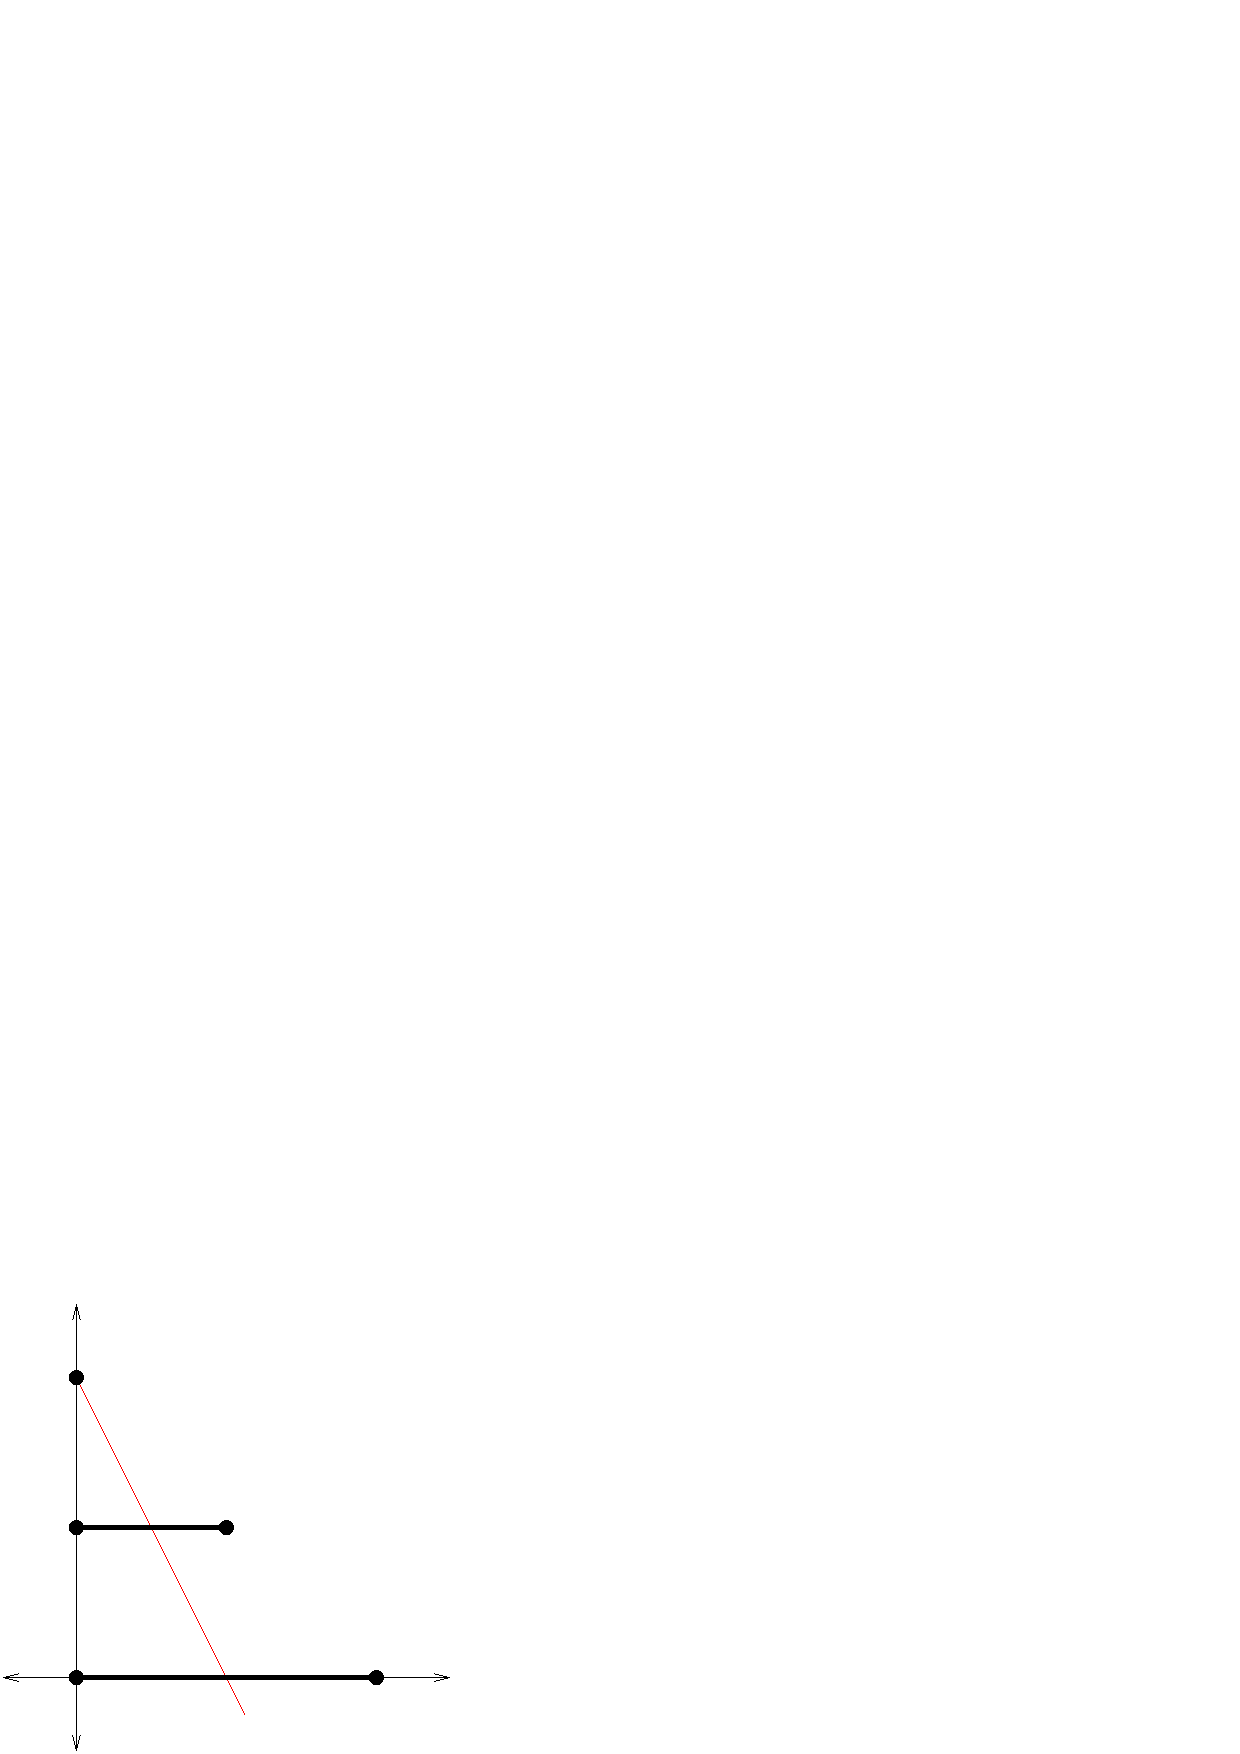
\includegraphics{figures/equiv_intervals.pdf}%
\end{picture}%
\setlength{\unitlength}{3947sp}%
%
\begingroup\makeatletter\ifx\SetFigFont\undefined%
\gdef\SetFigFont#1#2#3#4#5{%
  \reset@font\fontsize{#1}{#2pt}%
  \fontfamily{#3}\fontseries{#4}\fontshape{#5}%
  \selectfont}%
\fi\endgroup%
\begin{picture}(3624,3624)(1789,-3373)
\end{picture}%

\caption[Equivalent intervals.]{Projection from a point can be %
used to show that intervals of %
different lengths contain the same number of points.}
\label{fig:equiv_intervals} 
\end{figure}


By considering appropriate projections we can prove that any two arbitrary
intervals (say $[a, b]$ and $[c, d]$) have the same cardinalities!  It also
isn't all that hard to derive a formula for a bijective function between two
intervals.

\[ f(x) = c + \frac{(x - a)(d - c)}{(b - a)} \]

There are other geometric constructions which we can use to show that
there are the same number of points in a variety of entities.  For example,
consider the upper half of the unit circle (Remember the unit circle from
Trig?  All points $(x, y)$ satisfying $x^2 + y^2 = 1$.)  This is a 
semi-circle having a radius of 1, so the arclength of said semi-circle 
is $\pi$. It isn't hard to imagine
that this semi-circular arc contains the same number of points as an interval
of length $\pi$, and we've already argued that all intervals contain the same
number of points\ldots   But, a nice example of geometric projection ---  
vertical projection (a.k.a. $\pi_1$) ---  can be used to show that 
(for example) the interval
$(-1, 1)$ and the portion of the unit circle lying in the upper 
half-plane are equinumerous.

\begin{figure}[!hbtp]
\input{figures/interval_n_semicircle.tex}
\caption[An interval is equivalent to a semi-circle.]{Vertical projection %
provides a bijective correspondence between an interval and a semi-circle. }
\label{fig:interval_n_semicircle} 
\end{figure}

Once the bijection is understood geometrically it is fairly simple to provide
formulas.  To go from the semi-circle to the interval, we just forget
about the y-coordinate:

\[ f(x, y) = x. \]


To go in the other direction we need to recompute the missing y-value:

\[ f^{-1}(x) = (x, \sqrt{1 - x^2}).\]

Now we're ready to put some of these ideas together in order to prove
something really quite remarkable.  It may be okay to say that line segments
of different lengths are equinumerous -- although ones intuition still balks
at the idea that a line a mile long only has the same number of points on
it as a line an inch long (or, if you prefer, make that a centimeter versus
a kilometer).  Would you believe that the entire line -- that is the infinitely
extended line -- has no more points on it than a tiny little segment? You
should be ready to prove this one yourself.

\begin{exer}
Find a point such that projection from that point determines a
one-to-one correspondence between the portion of the unit circle in the upper
half plane and the line $y = 1$.  
\end{exer}

In the exercises from Section~\ref{sec:equiv_sets} you were supposed 
to show that set
equivalence is an equivalence relation.  Part of that proof should have been
showing that the relation is transitive, and that really just comes down to
showing that the composition of two bijections is itself a bijection.  If you
didn't make it through that exercise give it another try now, but whether
or not you can finish that proof it should be evident what that transitivity
means to us in the current situation.  Any pair of line segments are the same
size -- a line segment (i.e. an interval) and a semi-circle are the same size --
the semi-circle and an infinite line are the same size -- transitivity tells us that
an infinitely extended line has the same number of points as (for example)
the interval $(0, 1)$.

\clearpage

\noindent{\large \bf Exercises --- \thesection\ }

\input{card/examples-exer.tex}

\newpage

\section{Cantor's theorem}
\label{sec:cantors_thm}

Many people believe that the result known as Cantor's theorem says that
the real numbers, $\Reals$, have a greater cardinality than the natural numbers, $\Naturals$.
That isn't quite right.  In fact Cantor's theorem is a much broader statement,
one of whose consequences is that $|\Reals| > |\Naturals|$.  Before we go 
on to discuss Cantor's theorem in full generality, we'll first explore it, 
essentially, in this simplified form.
Once we know that $|\Reals| \neq |\Naturals|$, we'll be in a position to 
explore a lot of
interesting issues relative to the infinite.  In particular, this result 
means that there are at least two cardinal numbers that are 
infinite -- thus the ``infinity is infinity'' idea will be discredited.  
Once we have the full power of Cantor's
theorem, we'll see just how completely wrong that concept is.  

To show that some pair of sets are not equivalent it is necessary to show
that there cannot be a one-to-one correspondence between them.  Ordinarily,
one would try to argue by contradiction in such a situation.  That is what
we'll need to do to show that the reals and the naturals are not equinumerous.
We'll presume that they are in fact the same size and try to reach a
contradiction.

What exactly does the assumption that $\Reals$ and $\Naturals$ are 
equivalent mean?
It means there is a one-to-one correspondence, that is, a bijective function
from $\Reals$ to $\Naturals$.   In a nutshell, it means that it is 
possible to list all the real
numbers in a singly-infinite list.  Now, it is certainly possible to make an
infinite list of real numbers (since $\Naturals \subseteq \Reals$, 
by listing the naturals themselves
we are making an infinite list of reals!).  The problem is that we would need
to be sure that every real number is on the list somewhere.  In fact, since
we've used a geometric argument to show that the interval $(0, 1)$ and the 
set $\Reals$ are equinumerous, it will be sufficient to presume that there 
is an infinite list containing all the numbers in the interval $(0, 1)$.

\begin{exer}  Notice that, for example,  $\pi-3$ is a real number in 
$(0, 1)$.  Make
a list of $10$ real numbers in the interval $(0, 1)$.   Make sure that 
at least 5 of them are not rational.
\end{exer}

In the previous exercise, you've started the job, but we need to presume
that it is truly possible to complete this job.  That is, we must presume 
that there really is an infinite list containing every real number in 
the interval $(0, 1)$.

Once we have an infinite list containing every real number in the interval
$(0, 1)$ we have to face up to a second issue. What does it really mean
to list a particular real number? For instance if $e-2$ is in the seventh
position on our list, is it OK to write ``$e-2$'' there or should we write
``0.7182818284590452354\ldots''?  Clearly it would be simpler to write 
``$e-2$'' but it isn't necessarily possible to do something of that kind 
for every real
number -- on the other hand, writing down the decimal expansion is a problem
too; in a certain sense, ``most'' real numbers in (0, 1) have infinitely long
decimal expansions.  There is also another problem with decimal expansions;
they aren't unique.  For example, there is really no difference between the
finite expansion $0.5$ and the infinitely long expansion  $0.4\overline{9}$.

Rather than writing something like ``$e-2$'' or ``0.7182818284590452354\ldots'',
we are going to in fact write ``.1011011111100001010100010110001010001010 \ldots''
In other words, we are going to write the base-2 expansions of the real numbers
in our list. Now, the issue of non-uniqueness is still there in binary, and
in fact if we were to stay in base-10 it would be possible to plug a certain
gap in our argument -- but the binary version of this argument has some
especially nice features.
Every binary (or for that matter decimal) expansion corresponds to a unique 
real number, but it doesn't work out so well the other way around ---
there are sometimes two different binary expansions that correspond to the
same real number. There is a lovely fact that we are not going to prove (you
may get to see this result proved in a course in Real Analysis) that points up
the problem. Whenever two different binary expansions represent the same
real number, one of them is a terminating expansion (it ends in infinitely
many 0's) and the other is an infinite expansion (it ends in infinitely many
1's). We won't prove this fact, but the gist of the argument is a proof by
contradiction --- you may be able to get the point by studying Figure~\ref{fig:binary_reps}.
(Try to see how it would be possible to find a number in between two binary
expansions that didn't end in all-zeros and all-ones.)

\begin{figure}[!hbtp]
\begin{picture}(0,0)%
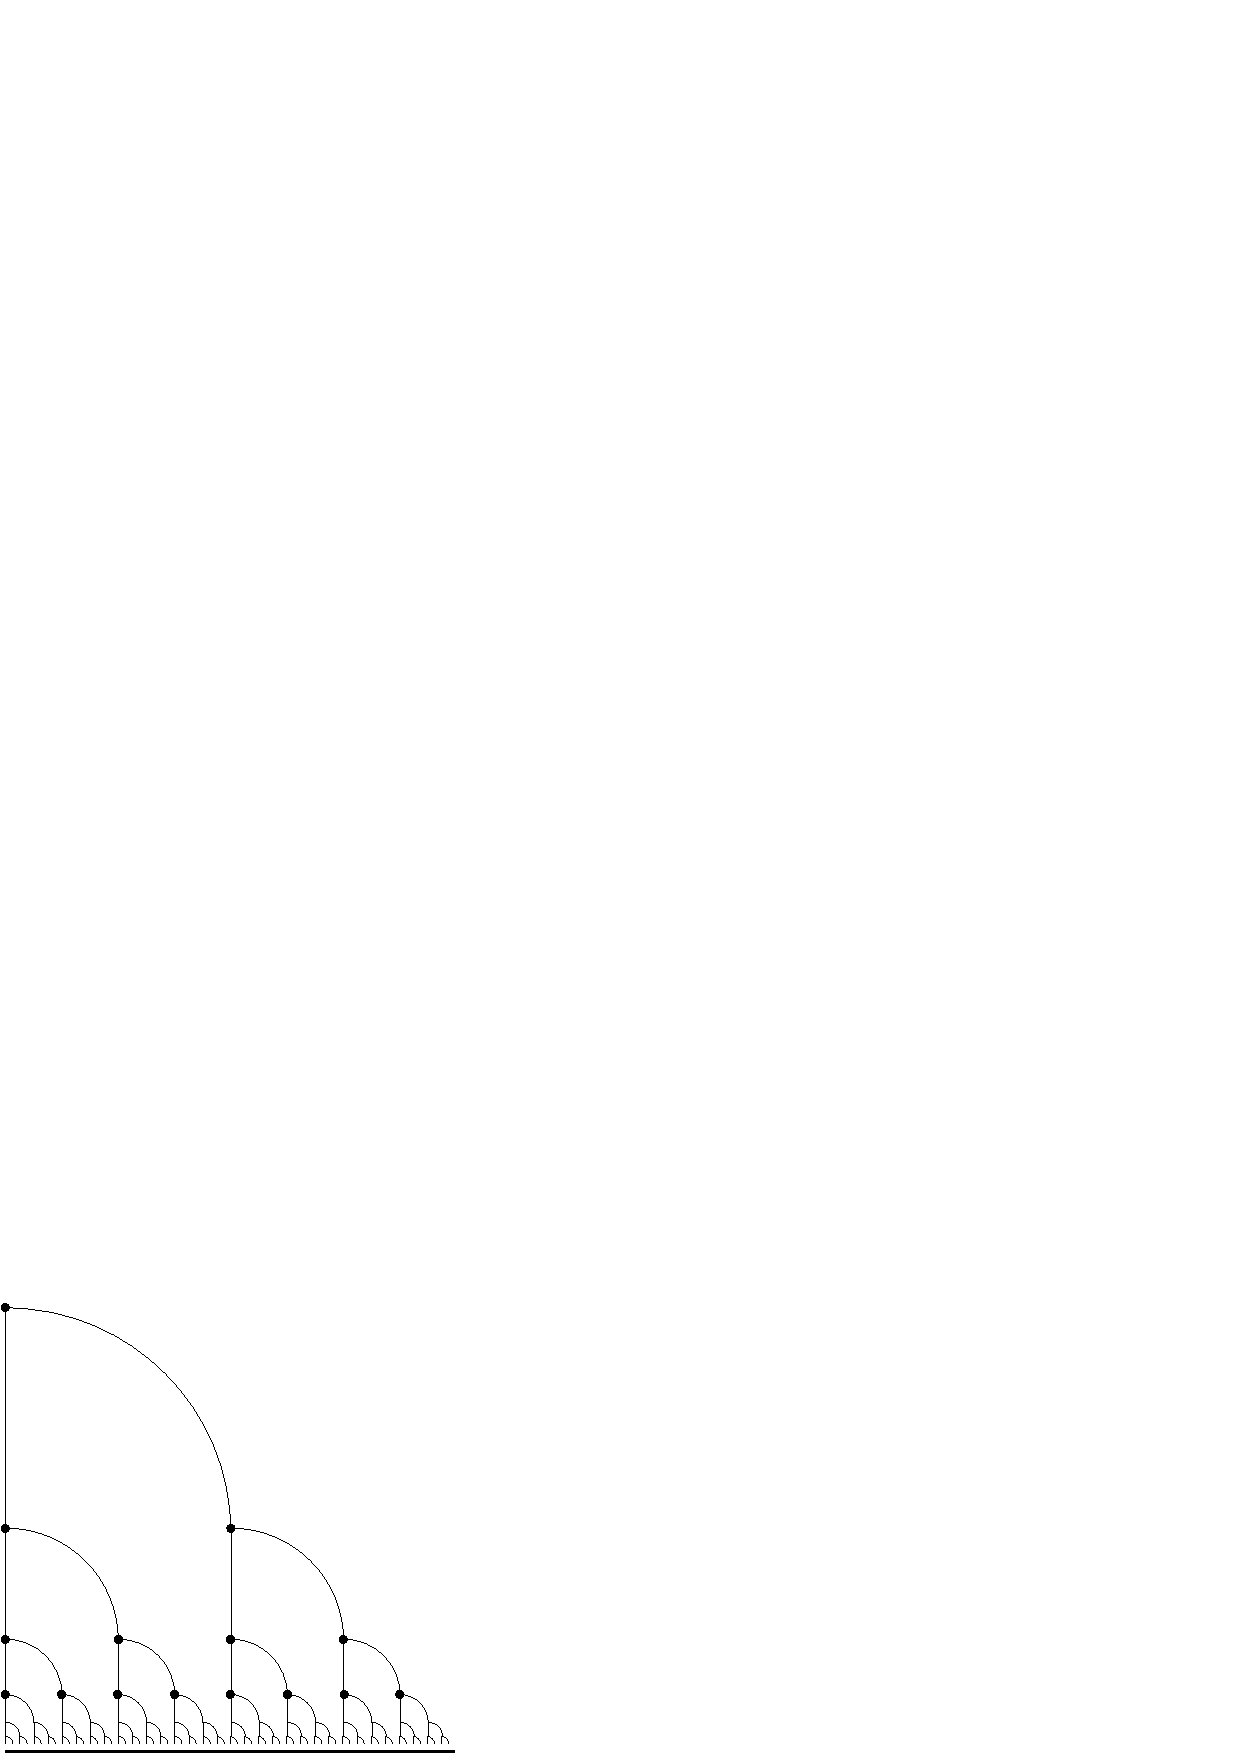
\includegraphics{./binary_reps.pdf}%
\end{picture}%
\setlength{\unitlength}{3947sp}%
%
\begingroup\makeatletter\ifx\SetFigFont\undefined%
\gdef\SetFigFont#1#2#3#4#5{%
  \reset@font\fontsize{#1}{#2pt}%
  \fontfamily{#3}\fontseries{#4}\fontshape{#5}%
  \selectfont}%
\fi\endgroup%
\begin{picture}(3656,3611)(2355,-4529)
\put(2449,-2637){\makebox(0,0)[lb]{\smash{{\SetFigFont{12}{14.4}{\familydefault}{\mddefault}{\updefault}{\color[rgb]{0,0,0}$.0$}%
}}}}
\put(2449,-3544){\makebox(0,0)[lb]{\smash{{\SetFigFont{12}{14.4}{\familydefault}{\mddefault}{\updefault}{\color[rgb]{0,0,0}$.00$}%
}}}}
\put(3356,-3544){\makebox(0,0)[lb]{\smash{{\SetFigFont{12}{14.4}{\familydefault}{\mddefault}{\updefault}{\color[rgb]{0,0,0}$.01$}%
}}}}
\put(4276,-3544){\makebox(0,0)[lb]{\smash{{\SetFigFont{12}{14.4}{\familydefault}{\mddefault}{\updefault}{\color[rgb]{0,0,0}$.10$}%
}}}}
\put(5176,-3544){\makebox(0,0)[lb]{\smash{{\SetFigFont{12}{14.4}{\familydefault}{\mddefault}{\updefault}{\color[rgb]{0,0,0}$.11$}%
}}}}
\put(4269,-2657){\makebox(0,0)[lb]{\smash{{\SetFigFont{12}{14.4}{\familydefault}{\mddefault}{\updefault}{\color[rgb]{0,0,0}$.1$}%
}}}}
\put(4668,-4009){\makebox(0,0)[lb]{\smash{{\SetFigFont{12}{14.4}{\familydefault}{\mddefault}{\updefault}{\color[rgb]{0,0,0}$.101$}%
}}}}
\put(5586,-4010){\makebox(0,0)[lb]{\smash{{\SetFigFont{12}{14.4}{\familydefault}{\mddefault}{\updefault}{\color[rgb]{0,0,0}$.111$}%
}}}}
\put(5128,-4003){\makebox(0,0)[lb]{\smash{{\SetFigFont{12}{14.4}{\familydefault}{\mddefault}{\updefault}{\color[rgb]{0,0,0}$.110$}%
}}}}
\put(3770,-4014){\makebox(0,0)[lb]{\smash{{\SetFigFont{12}{14.4}{\familydefault}{\mddefault}{\updefault}{\color[rgb]{0,0,0}$.011$}%
}}}}
\put(4225,-4005){\makebox(0,0)[lb]{\smash{{\SetFigFont{12}{14.4}{\familydefault}{\mddefault}{\updefault}{\color[rgb]{0,0,0}$.100$}%
}}}}
\put(3324,-4009){\makebox(0,0)[lb]{\smash{{\SetFigFont{12}{14.4}{\familydefault}{\mddefault}{\updefault}{\color[rgb]{0,0,0}$.010$}%
}}}}
\put(2878,-4009){\makebox(0,0)[lb]{\smash{{\SetFigFont{12}{14.4}{\familydefault}{\mddefault}{\updefault}{\color[rgb]{0,0,0}$.001$}%
}}}}
\put(2423,-4004){\makebox(0,0)[lb]{\smash{{\SetFigFont{12}{14.4}{\familydefault}{\mddefault}{\updefault}{\color[rgb]{0,0,0}$.000$}%
}}}}
\end{picture}%

\caption[Binary representations in the unit interval.]{The base-$2$ %
expansions of reals in the interval $[0, 1]$ are the leaves of an %
infinite tree.}
\label{fig:binary_reps} 
\end{figure}

So, instead of showing that the set of reals in $(0, 1)$ can't be put 
in one-to-one
correspondence with $\Naturals$, what we're really going to do is show 
that their binary expansions can't be put in one-to-one correspondence 
with $\Naturals$.  Since
there are an infinite number of reals that have two different binary expansions
this doesn't really do the job as advertised at the beginning of this section.
(Perhaps you are getting used to our wily ways by now --- yes, this does
mean that we're going to ask you to do the real proof in the exercises.)
The set of binary numerals, $\{0, 1\}$, is an instance of a mathematical 
structure known as a field; basically, that means that it's possible to 
add, subtract, multiply and divide (but not divide by 0) with them. 
We are only mentioning this fact so that you'll understand why the set 
$\{0, 1\}$ is often referred to as ${\mathbb F}_2$.  We're only mentioning that 
fact so that you'll understand why we call the set of all possible 
binary expansion ${\mathbb F}_2^\infty$ .  Finally, we're only mentioning \emph{that} 
fact so that we'll have a succinct way of expressing this set.  
Now we can write ``${\mathbb F}_2^\infty$'' rather than 
``the set of all possible infinitely-long binary sequences.''

Suppose we had a listing of all the elements of ${\mathbb F}_2^\infty$.  We would have an
infinite list of things, each of which is itself an infinite list 
of 0's and 1's.

So what? We need to proceed from here to find a contradiction.

This argument that we've been edging towards is known as Cantor's 
diagonalization argument. The reason for this name is that our 
listing of binary representations looks like an enormous table 
of binary digits and the contradiction is deduced by looking at 
the diagonal of this infinite-by-infinite table.
The diagonal is itself an infinitely long binary string --- in other words, the
diagonal can be thought of as a binary expansion itself.  
If we take the complement
of the diagonal, (switch every 0 to a 1 and vice versa) we will also
have a thing that can be regarded as a binary expansion and this binary
expansion can't be one of the ones on the list!  This bit-flipped version of
the diagonal is different from the first binary expansion in the first 
position,
it is different from the second binary expansion in the second position, it is
different from the third binary expansion in the third position, and so on.
The very presumption that we could list all of the elements of ${\mathbb F}_2^\infty$ 
allows us
to construct an element of ${\mathbb F}_2^\infty$ that could not be on the list!

This argument has been generalized many times, so this is the first in a
class of things known as diagonal arguments.  Diagonal arguments have been
used to settle several important mathematical questions.  There is a valid
diagonal argument that even does what we'd originally set out to do: prove
that $\Naturals$  and $\Reals$ are not equinumerous.  Strangely, the 
argument can't be made to work in binary, and since you're going to be 
asked to write it up in the exercises, we want to point out one of the 
potential pitfalls.
If we were to use a diagonal argument to show that $(0, 1)$ isn't countable,
we would start by assuming that every element of $(0, 1)$ was written down in
a list. For most real numbers in $(0, 1)$ we could write out their 
binary representation uniquely, but for some we would have to make a 
choice: should we write down the representation that terminates, or 
the one that ends in infinitely-many 1's?  Suppose we choose to use 
the terminating representations, then none of the infinite binary 
strings that end with all 1's will be on the list. It's possible that 
the thing we get when we complement the diagonal
is one of these (unlisted) binary strings so we don't \emph{necessarily} 
have a contradiction.
If we make the other choice -- use the infinite binary representation
when we have a choice -- there is a similar problem.
You may think that our use of binary representations for real numbers
was foolish in light of the failure of the argument to ``go through'' 
in binary.
Especially since, as we've alluded to, it can be made to work in decimal.
The reason for our apparent stubbornness is that these infinite binary
strings do something else that's very nice.  An infinitely long binary sequence
can be thought of as the indicator function of a subset of N. For example,
$.001101010001$ is the indicator of $\{2, 3, 5, 7, 11\}$.

\begin{exer} 

Complete the table.
\medskip

\begin{center}
\begin{tabular}{l|l}
binary expansion & subset of $\Naturals$ \\ \hline\hline
\rule[-4pt]{0pt}{20pt} $.1$ & $\{0\}$ \\\hline
\rule[-4pt]{0pt}{20pt}$.0111$ &   \\\hline
\rule[-4pt]{0pt}{20pt} & $\{2, 4, 6\}$ \\\hline
\rule[-4pt]{0pt}{20pt}$.\overline{01}$ & \\\hline
\rule[-4pt]{0pt}{20pt} & $\{3k + 1 \suchthat k \in \Naturals\}$ \\
\end{tabular}
\end{center}

\end{exer}


The set, ${\mathbb F}_2^\infty$, we've been working with is in one-to-one correspondence
with the power set of the natural numbers, ${\mathcal P}(\Naturals)$.  
When viewed in this light, the proof we did above showed that the power 
set of $\Naturals$ has an infinite cardinality strictly greater than that 
of $\Naturals$ itself.  In other words, ${\mathcal P}(\Naturals)$ is
uncountable.

What Cantor's theorem says is that this always works. If $A$ is any set,
and ${\mathcal P}(A)$ is its power set then $|A| < |{\mathcal P}(A)|$. 
In a way, this more general
theorem is easier to prove than the specific case we just handled.

\begin{thm}[Cantor]  
For all sets $A$, $A$ is not equivalent to ${\mathcal P}(A)$.
\end{thm}

\begin{proof}
Suppose that there is a set $A$ that can be placed in one-to-one
correspondence with its power set.  Then there is a bijective
function $f : A \longrightarrow {\mathcal P}(A)$.  We will deduce 
a contradiction by constructing a subset of $A$ 
(i.e. a member of ${\mathcal P}(A))$ that cannot
be in the range of $f$.

Let $S = \{x \in A \suchthat x \notin f(x)\}$.

If $S$ is in the range of $f$, there is a preimage $y$ such that $S = f(y)$.
But, if such a $y$ exists then the membership question, $y \in S$, must
either be true or false.   If $y \in S$,  then because $S = f(y)$, and $S$
consists of those elements that are not in their images, it follows
that $y \notin S$.  On the other hand, if $y \notin S$ then $y \notin f(y)$ so 
(by the definition of $S$) it follows that $y \in S$.  Either possibility leads to the other, which is a contradiction.
\end{proof}

Cantor's theorem guarantees that there is an infinite hierarchy of infinite
cardinal numbers.  Let's put it another way.  People have sought a construction
that, given an infinite set, could be used to create a strictly larger set.  
For
instance, the Cartesian product works like this if our sets are finite --- 
$A \times A$ is strictly bigger than $A$ when $A$ is a finite set.  But, as 
we've already seen,
this is not necessarily so if $A$ is infinite (remember the ``snake'' argument
that $\Naturals$ and $\Naturals \times \Naturals$ are equivalent).  The 
real import of Cantor's theorem is that taking the power set of a set 
\emph{does} create a set of larger cardinality.
So we get an infinite tower of infinite cardinalities, starting with 
$\aleph_0 = |\Naturals|$, by successively taking power sets.

\[ \aleph_0  = |\Naturals| < |{\mathcal P}(\Naturals)| < |{\mathcal P}({\mathcal P}(\Naturals))| < |{\mathcal P}({\mathcal P}({\mathcal P}(\Naturals)))| < \ldots \]

\clearpage

\noindent{\large \bf Exercises --- \thesection\ }

\begin{enumerate}
\item Determine a substitution rule -- a consistent way of replacing one digit
with another along the diagonal so that a diagonalization proof showing
that the interval (0, 1) is uncountable will work in decimal. Write up
the proof.

\wbvfill

\item Can a diagonalization proof showing that the interval (0, 1) is uncountable
be made workable in base-3 (ternary) notation?

\wbvfill

\workbookpagebreak

\item In the proof of Cantor's theorem we construct a set $S$ that cannot
be in the image of a presumed bijection from $A$ to ${\mathcal P}(A)$.  
Suppose $A = \{1, 2, 3\}$ and f determines the following correspondences: 
$1 \longleftrightarrow \emptyset$,
$2 \longleftrightarrow \{1, 3\}$ and $3 \longleftrightarrow \{1, 2, 3\}$. 
What is $S$?

\wbvfill

\item An argument very similar to the one embodied in the proof of Cantor's
theorem is found in the Barber's paradox. This paradox was
originally introduced in the popular press in order to give laypeople an
understanding of Cantor's theorem and Russell's paradox. It sounds
somewhat sexist to modern ears. (For example, it is presumed without
comment that the Barber is male.)

\begin{quote}
In a small town there is a Barber who shaves those men (and
only those men) who do not shave themselves. Who shaves
the Barber?
\end{quote}

Explain the similarity to the proof of Cantor's theorem.

\wbvfill

\workbookpagebreak

\item Cantor's theorem, applied to the set of all sets leads to an interesting
paradox. The power set of the set of all sets is a collection of sets, so
it must be contained in the set of all sets. Discuss the paradox and
determine a way of resolving it.

\wbvfill

\item Verify that the final deduction in the proof of Cantor's theorem, 
``$(y \in S  \implies  y \notin S) \land  (y \notin S \implies y \in S)$,'' 
is truly a contradiction.

\wbvfill

\workbookpagebreak

\end{enumerate}

%% Emacs customization
%% 
%% Local Variables: ***
%% TeX-master: "GIAM-hw.tex" ***
%% comment-column:0 ***
%% comment-start: "%% "  ***
%% comment-end:"***" ***
%% End: ***



\newpage

\section{Dominance}
\label{sec:dominance}

We've said a lot about the equivalence relation 
determined by Cantor's definition
of set equivalence.  We've also, occasionally, written things like 
$|A| < |B|$, without being particularly clear about what that means.  
It's now time to come clean.  There is actually a (perhaps) more fundamental 
notion used for comparing set sizes than equivalence --- dominance. 
Dominance is an ordering relation on the class of all sets.  
One should probably really define dominance first and then
define set equivalence in terms of it.  We haven't followed that plan
for (at least) two reasons.   First, many people may want to skip this 
section --- the results of this section depend on the difficult 
Cantor-Bernstein-Schr\"{o}der theorem\footnote{This theorem has been %
known for many years as the Schr\"{o}der-Bernstein theorem, but, %
lately, has had Cantor's name added as well. Since Cantor proved % 
the result before the other gentlemen this is fitting. It is also %
known as the Cantor-Bernstein theorem (leaving out Schr\"{o}der) %
which doesn't seem very nice.}.  Second, we will later take the view that dominance
should really be considered to be an ordering relation on the set of
all cardinal numbers -- i.e. the equivalence classes of the set equivalence
relation -- not on the collection of all sets.  From that perspective,
set equivalence really needs to be defined \emph{before} dominance.

One set is said to dominate another if there is a function from the latter
\emph{into} the former.
More formally, we have the following

\begin{defi}  If $A$ and $B$ are sets, we say ``$A$ dominates $B$'' 
and write $|A| > |B|$ iff there is an injective function $f$ with 
domain $B$ and codomain $A$.
\end{defi}

It is easy to see that this relation is reflexive and transitive.  The Cantor-
Bernstein-Schr\"{o}der theorem proves that it is also anti-symmetric --- which
means dominance is an ordering relation.  Be advised that there is an abuse
of terminology here that one must be careful about --- what are the domain
and range of the ``dominance'' relation?  The definition would lead us to
think that sets are the things that go on either side of the ``dominance''
relation, but the notation is a bit more honest, ``$|A| > |B|$'' 
indicates that the
things really being compared are the cardinal numbers of sets (not the sets
themselves).  Thus anti-symmetry for this relation is

\[ (|A| > |B|) \land (|B| > |A|) \implies (|A| = |B|). \]

In other words, if $A$ dominates $B$ and vice versa, then $A$ and $B$ are
equivalent sets --- a strict interpretation of anti-symmetry for this relation
might lead to the conclusion that $A$ and $B$ are actually the same set, which
is clearly an absurdity.

Naturally, we want to prove the Cantor-Bernstein-Schr\"{o}der theorem (which
we're going to start calling the C-B-S theorem for brevity), but first it'll be
instructive to look at some of its consequences. Once we have the C-B-S
theorem we get a very useful shortcut for proving set equivalences. Given
sets $A$ and $B$, if we can find injective functions going between them in both
directions, we'll know that they're equivalent. So, for example, we can use
C-B-S to prove that the set of all infinite binary strings and the set of reals
in (0, 1) really are equinumerous.  
(In case you had some remaining doubt\ldots )

It is easy to dream up an injective function from $(0, 1)$ 
to ${\mathbb F}_2^\infty$ : just send a
real number to its binary expansion, and if there are two, make a consistent
choice --- let's say we'll take the non-terminating expansion.

There is a cute thought-experiment called Hilbert's Hotel that will lead
us to a technique for developing an injective function in the other direction.
Hilbert's Hotel has $\aleph_0$ rooms. If any countable collection of 
guests show up there will be enough rooms for everyone.   Suppose you 
arrive at Hilbert's hotel one dark and stormy evening and the 
``No Vacancy'' light is on --- there are already a
denumerable number of guests there --- every room is full. The clerk 
sees you dejectedly considering your options, trying to think of 
another hotel that might still have rooms when, clearly, a \emph{very} 
large convention is in town.  He rushes out and says 
``My friend, have no fear! Even though we have no vacancies,
there is always room for one more at our establishment.''  
He goes into the office and makes the following announcement 
on the PA system.  ``Ladies and Gentlemen, in order to accommodate 
an incoming guest, please vacate your room and move to the room 
numbered one higher. Thank you.''  There
is an infinite amount of grumbling, but shortly you find yourself occupying
room number $1$.

To develop an injection from ${\mathbb F}_2^\infty$ to $(0, 1)$ we'll use ``room number 1'' to
separate the binary expansions that represent the same real number.  Move
all the digits of a binary expansion down by one, and make the first digit
$0$ for (say) the terminating expansions and $1$ for the non-terminating ones.
Now consider these expansions as real numbers --- all the expansions that
previously coincided are now separated into the intervals $(0, 1/2)$ and 
$(1/2, 1)$.  Notice how funny this map is, there are now 
many, many, (infinitely-many) 
real numbers with no preimages.  For instance, only a subset of the rational
numbers in $(0, 1/2)$ have preimages. Nevertheless, the map is injective, so
C-B-S tells us that ${\mathbb F}_2^\infty$ and $(0, 1)$ are equivalent.
There are quite a few different proofs of the C-B-S theorem. The one
Cantor himself wrote relies on the axiom of choice.  The axiom of choice
was somewhat controversial when it was introduced, but these days most
mathematicians will use it without qualms.  What it says (essentially) is that
it is possible to make an infinite number of choices.  More precisely, it says
that if we have an infinite set consisting of non-empty sets, it is possible
to select an element out of each set.  If there is a definable rule for picking
such an element (as is the case, for example, when we selected the 
nonterminating decimal expansion whenever there was a choice in defining the
injection from $(0, 1)$ to ${\mathbb F}_2^\infty$) the axiom of choice 
isn't needed.   The usual
axioms for set theory were developed by Zermelo and Frankel, so you may
hear people speak of the ZF axioms.  If, in addition, we want to specifically
allow the axiom of choice, we are in the ZFC axiom system.  If it's possible
to construct a proof for a given theorem without using the axiom of choice,
almost everyone would agree that that is preferable.  On the other hand,
a proof of the C-B-S theorem, which necessarily must be able to deal with
uncountably infinite sets, will have to depend on some sort of notion that
will allow us to deal with huge infinities.

The proof we will present here\footnote{We first encountered this proof 
in a Wikipedia article\cite{wiki-CBS}.} is attributed to Julius K\"{o}nig.  
K\"{o}nig was a contemporary of Cantor's who was (initially) very 
much respected by him.  Cantor came to dislike K\"{o}nig after the 
latter presented a well-publicized (and ultimately wrong) lecture 
claiming the continuum hypothesis was false.
Apparently the continuum hypothesis was one of Cantor's favorite ideas,
because he seems to have construed K\"{o}nig's lecture as a personal attack.
Anyway\ldots 

K\"{o}nig's proof of C-B-S doesn't use the axiom of choice, but it does have
its own strangeness: a function that is not necessarily computable --- that is,
a function for which (for certain inputs) it may not be possible to compute
an output in a finite amount of time!  Except for this oddity, 
K\"{o}nig's proof
is probably the easiest to understand of all the proofs of C-B-S. 
Before we get too far into the proof it is essential that we understand the
basic setup.  The Cantor-Bernstein-Schr\"{o}der theorem states that 
whenever $A$
and $B$ are sets and there are injective functions 
$f : A \longrightarrow B$ and $g : B \longrightarrow A$,
then it follows that $A$ and $B$ are equivalent.  Saying $A$ and $B$ 
are equivalent
means that we can find a bijective function between them.  So, to prove 
C-B-S, we hypothesize the two injections and somehow we must construct the
bijection.

\begin{figure}[!hbtp]
\begin{center}
\begin{picture}(0,0)%
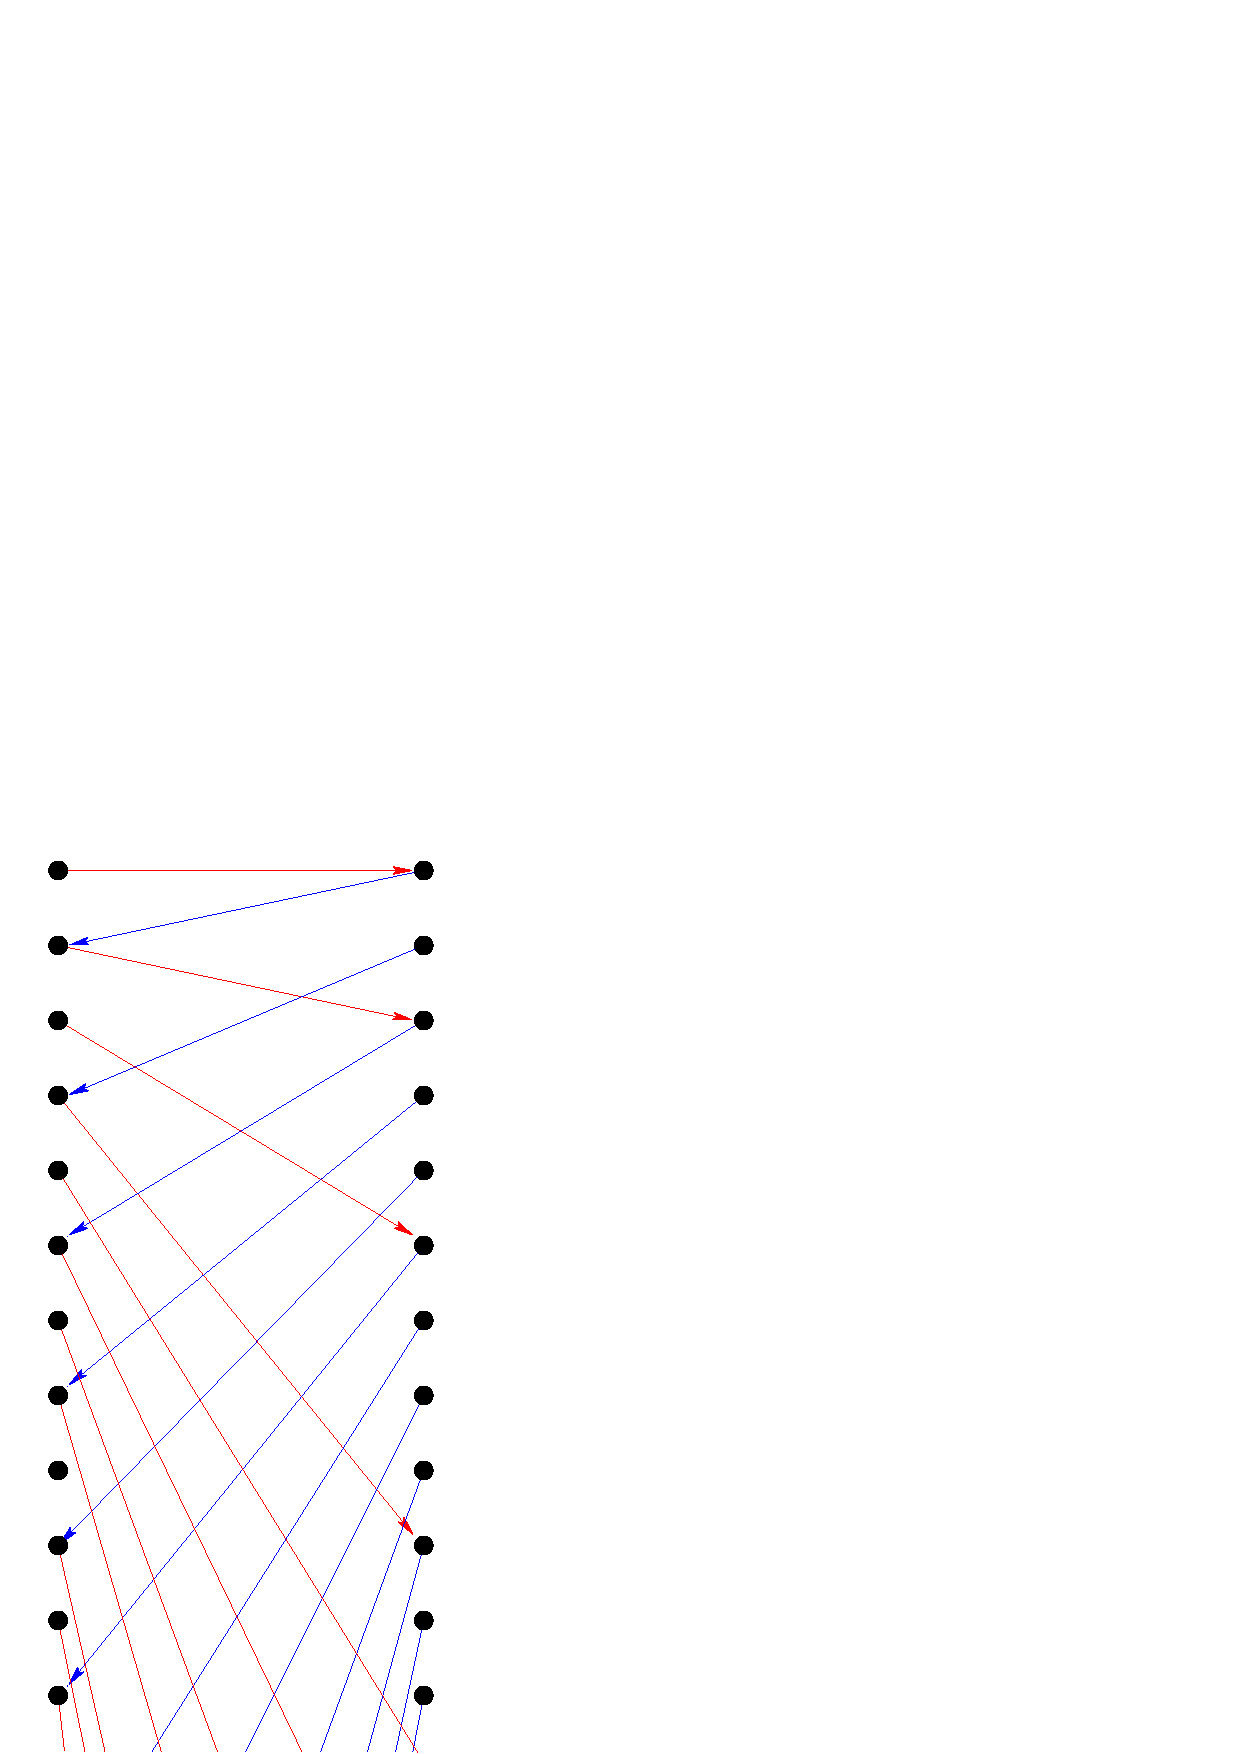
\includegraphics{./CBS_setup.pdf}%
\end{picture}%
\setlength{\unitlength}{3947sp}%
%
\begingroup\makeatletter\ifx\SetFigFont\undefined%
\gdef\SetFigFont#1#2#3#4#5{%
  \reset@font\fontsize{#1}{#2pt}%
  \fontfamily{#3}\fontseries{#4}\fontshape{#5}%
  \selectfont}%
\fi\endgroup%
\begin{picture}(3555,7591)(1186,-7730)
\put(4726,-736){\makebox(0,0)[lb]{\smash{{\SetFigFont{12}{14.4}{\familydefault}{\mddefault}{\updefault}{\color[rgb]{0,0,0}$b_1$}%
}}}}
\put(4726,-1336){\makebox(0,0)[lb]{\smash{{\SetFigFont{12}{14.4}{\familydefault}{\mddefault}{\updefault}{\color[rgb]{0,0,0}$b_2$}%
}}}}
\put(4726,-1936){\makebox(0,0)[lb]{\smash{{\SetFigFont{12}{14.4}{\familydefault}{\mddefault}{\updefault}{\color[rgb]{0,0,0}$b_3$}%
}}}}
\put(4726,-2536){\makebox(0,0)[lb]{\smash{{\SetFigFont{12}{14.4}{\familydefault}{\mddefault}{\updefault}{\color[rgb]{0,0,0}$b_4$}%
}}}}
\put(4726,-3136){\makebox(0,0)[lb]{\smash{{\SetFigFont{12}{14.4}{\familydefault}{\mddefault}{\updefault}{\color[rgb]{0,0,0}$b_5$}%
}}}}
\put(4726,-3736){\makebox(0,0)[lb]{\smash{{\SetFigFont{12}{14.4}{\familydefault}{\mddefault}{\updefault}{\color[rgb]{0,0,0}$b_6$}%
}}}}
\put(4726,-4336){\makebox(0,0)[lb]{\smash{{\SetFigFont{12}{14.4}{\familydefault}{\mddefault}{\updefault}{\color[rgb]{0,0,0}$b_7$}%
}}}}
\put(4726,-4936){\makebox(0,0)[lb]{\smash{{\SetFigFont{12}{14.4}{\familydefault}{\mddefault}{\updefault}{\color[rgb]{0,0,0}$b_8$}%
}}}}
\put(4726,-5536){\makebox(0,0)[lb]{\smash{{\SetFigFont{12}{14.4}{\familydefault}{\mddefault}{\updefault}{\color[rgb]{0,0,0}$b_9$}%
}}}}
\put(4726,-6136){\makebox(0,0)[lb]{\smash{{\SetFigFont{12}{14.4}{\familydefault}{\mddefault}{\updefault}{\color[rgb]{0,0,0}$b_{10}$}%
}}}}
\put(4726,-6736){\makebox(0,0)[lb]{\smash{{\SetFigFont{12}{14.4}{\familydefault}{\mddefault}{\updefault}{\color[rgb]{0,0,0}$b_{11}$}%
}}}}
\put(4726,-7336){\makebox(0,0)[lb]{\smash{{\SetFigFont{12}{14.4}{\familydefault}{\mddefault}{\updefault}{\color[rgb]{0,0,0}$b_{12}$}%
}}}}
\put(1201,-736){\makebox(0,0)[lb]{\smash{{\SetFigFont{12}{14.4}{\familydefault}{\mddefault}{\updefault}{\color[rgb]{0,0,0}$a_1$}%
}}}}
\put(1201,-1336){\makebox(0,0)[lb]{\smash{{\SetFigFont{12}{14.4}{\familydefault}{\mddefault}{\updefault}{\color[rgb]{0,0,0}$a_2$}%
}}}}
\put(1201,-1936){\makebox(0,0)[lb]{\smash{{\SetFigFont{12}{14.4}{\familydefault}{\mddefault}{\updefault}{\color[rgb]{0,0,0}$a_3$}%
}}}}
\put(1201,-2536){\makebox(0,0)[lb]{\smash{{\SetFigFont{12}{14.4}{\familydefault}{\mddefault}{\updefault}{\color[rgb]{0,0,0}$a_4$}%
}}}}
\put(1201,-3136){\makebox(0,0)[lb]{\smash{{\SetFigFont{12}{14.4}{\familydefault}{\mddefault}{\updefault}{\color[rgb]{0,0,0}$a_5$}%
}}}}
\put(1201,-3736){\makebox(0,0)[lb]{\smash{{\SetFigFont{12}{14.4}{\familydefault}{\mddefault}{\updefault}{\color[rgb]{0,0,0}$a_6$}%
}}}}
\put(1201,-4336){\makebox(0,0)[lb]{\smash{{\SetFigFont{12}{14.4}{\familydefault}{\mddefault}{\updefault}{\color[rgb]{0,0,0}$a_7$}%
}}}}
\put(1201,-4936){\makebox(0,0)[lb]{\smash{{\SetFigFont{12}{14.4}{\familydefault}{\mddefault}{\updefault}{\color[rgb]{0,0,0}$a_8$}%
}}}}
\put(1201,-5536){\makebox(0,0)[lb]{\smash{{\SetFigFont{12}{14.4}{\familydefault}{\mddefault}{\updefault}{\color[rgb]{0,0,0}$a_9$}%
}}}}
\put(1201,-6136){\makebox(0,0)[lb]{\smash{{\SetFigFont{12}{14.4}{\familydefault}{\mddefault}{\updefault}{\color[rgb]{0,0,0}$a_{10}$}%
}}}}
\put(1201,-6736){\makebox(0,0)[lb]{\smash{{\SetFigFont{12}{14.4}{\familydefault}{\mddefault}{\updefault}{\color[rgb]{0,0,0}$a_{11}$}%
}}}}
\put(1201,-7336){\makebox(0,0)[lb]{\smash{{\SetFigFont{12}{14.4}{\familydefault}{\mddefault}{\updefault}{\color[rgb]{0,0,0}$a_{12}$}%
}}}}
\put(1576,-286){\makebox(0,0)[lb]{\smash{{\SetFigFont{12}{14.4}{\rmdefault}{\mddefault}{\updefault}{\color[rgb]{0,0,0}$A$}%
}}}}
\put(4501,-286){\makebox(0,0)[lb]{\smash{{\SetFigFont{12}{14.4}{\rmdefault}{\mddefault}{\updefault}{\color[rgb]{0,0,0}$B$}%
}}}}
\end{picture}%

\end{center}
\caption[Setup for proving the C-B-S theorem.]{Hypotheses for %
proving the Cantor-Bernstein-Schr\"{o}der theorem: %
two sets with injective functions going both ways.}
\label{fig:CBS_setup} 
\end{figure}

Figure~\ref{fig:CBS_setup} has a presumption in it --- 
that $A$ and $B$ are countable --- which
need not be the case.  Nevertheless, it gives us a good picture to work from.
The basic hypotheses, that $A$ and $B$ are sets and we have two functions, one
from $A$ into $B$ and another from $B$ into A, are shown.  
We will have to build our bijective function in a piecewise manner.
If there is a non-empty intersection between $A$ and $B$, we can use the
identity function for that part of the domain of our bijection.  
So, without
loss of generality, we can presume that $A$ and $B$ are disjoint.  
We can use
the functions $f$ and $g$ to create infinite sequences, which 
alternate back and
forth between $A$ and $B$, containing any particular element.
Suppose  $a \in A$ is an arbitrary element.  Since $f$ is defined 
on all of $A$, we
can compute $f(a)$.  Now since $f(a)$ is an element of $B$, and $g$ is 
defined on all
of $B$, we can compute $g(f(a))$, and so on.  Thus, we get the 
infinite sequence

\[ \rule{120pt}{0pt} a, \quad  f(a), \quad g(f(a)), \quad f(g(f(a))), \; \ldots \]

If the element $a$ also happens to be the image of something under $g$ (this
may or may not be so --- since $g$ isn't necessarily onto) then we 
can also extend
this sequence to the left.  Indeed, it may be possible to 
extend the sequence infinitely far to the left, or, this 
process may stop when one of $f^{-1}$ or $g^{-1}$
fails to be defined. 

\[
\ldots \; g^{-1}(f^{-1}(g^{-1}(a))), \quad f^{-1}(g^{-1}(a)), \quad g^{-1}(a), \quad a, \quad  f(a), \quad  g(f(a)), \quad f(g(f(a))),\; \ldots \]

Now, every element of the disjoint union of $A$ and $B$ is in one of these
sequences. Also, it is easy to see that these sequences are either disjoint
or identical. Taking these two facts together it follows that these sequences
form a partition of $A \cup B$.  We'll define a bijection  
$\phi : A \longrightarrow B$ by deciding what it must do on these 
sequences.  There are four possibilities for how the sequences we've 
just defined can play out. In extending them to the left, we may run 
into a place where one of the inverse functions needed isn't 
defined --- or not.  We say a sequence is an 
$A$-stopper, if, in extending to the left, we end 
up on an element of $A$ that has
no preimage under $g$ (see Figure~\ref{fig:A-stopper}).  Similarly, 
we can define a $B$-stopper.
If the inverse functions are always defined within a given sequence there are
also two possibilities; the sequence may be finite (and so it must be cyclic in
nature) or the sequence may be truly infinite.

\begin{figure}[!hbtp]
\begin{center}
\input{figures/A-stopper.tex}
\end{center}
\caption[An \emph{A}-stopper in the proof of C-B-S.]{An $A$-stopper
is an infinite sequence that terminates to the left in A.}
\label{fig:A-stopper} 
\end{figure}


Finally, here is a definition for $\phi$.

\[ \phi(x) =  \left\{ \begin{array}{cl} g^{-1}(x) & \mbox{if $x$ is in a $B$-stopper} \\ f(x) & \mbox{otherwise} \end{array} \right. \]

Notice that if a sequence is either cyclic or infinite it doesn't matter
whether we use $f$ or $g^{-1}$ since both will be 
defined for all elements of such
sequences.  Also, certainly $f$ will work if we are in an $A$-stopper.  
The function  we've just created is perfectly well-defined, but it may take
arbitrarily long to determine whether we have an element of a $B$-stopper, as
opposed to an element of an infinite sequence.  We cannot determine whether
we're in an infinite versus a finite sequence in a prescribed finite number of
steps.


\clearpage

\noindent{\large \bf Exercises --- \thesection\ }

\begin{enumerate}
\item How could the clerk at the Hilbert Hotel accommodate a countable
number of new guests?

\wbvfill

\item Let $F$ be the collection of all real-valued functions 
defined on the real line.  Find an injection from $\Reals$ to $F$.  Do you 
think it is possible to find an injection going the other way?  In 
other words, do you think that $F$ and $\Reals$ are equivalent?  Explain.

\wbvfill

\workbookpagebreak

\item Fill in the details of the proof that dominance is an ordering relation.
(You may simply cite the C-B-S theorem in proving anti-symmetry.)

\wbvfill

\item We can inject $\Rationals$ into $\Integers$ by sending 
$\displaystyle \pm \frac{a}{b}$ to $\displaystyle \pm 2^a3^b$.  
 Use this and another obvious injection to (in light of the C-B-S 
theorem) reaffirm the equivalence of these sets.

\wbvfill

\end{enumerate}

%% Emacs customization
%% 
%% Local Variables: ***
%% TeX-master: "GIAM-hw.tex" ***
%% comment-column:0 ***
%% comment-start: "%% "  ***
%% comment-end:"***" ***
%% End: ***



\newpage

\section[CH and GCH]{The continuum hypothesis and the generalized continuum hypothesis}
\label{sec:ch_gch}

The word ``continuum'' in the title of this section is used to indicate sets of
points that have a certain continuity property. For example, in a real interval
it is possible to move from one point to another, in a smooth fashion, without
ever leaving the interval. In a range of rational numbers this is not possible,
because there are irrational values in between every pair of rationals. There
are many sets that behave as a continuum -- the intervals (a, b) or [a, b], the
entire real line $\Reals$, the x-y plane $\Reals \times \Reals$, a volume in 3-dimensional space (or
for that matter the entire space $\Reals^3$). It turns out that all of these sets have
the same size.

The cardinality of the continuum, denoted {\bf c}, is the cardinality of all of the
sets above. 

In the previous section we mentioned the continuum hypothesis and how
angry Cantor became when someone (K\"{o}nig) tried to prove it
was false.   In this section we'll delve a little deeper into what the
continuum hypothesis says and even take a look at CH's big brother, GCH.
Before doing so, it seems like a good idea to look into the equivalences
we've asserted about all those sets above which (if you trust us) have the
cardinality {\bf c}.

We've already seen that an interval is equivalent to the entire
real line but the notion that the entire infinite Cartesian plane has no more
points in it than an interval one inch long defies our intuition. Our conception
of dimensionality leads us to think that things of higher dimension must be
larger than those of lower dimension. This preconception is false as we can see
by demonstrating that a $1 \times 1$  square can be put in one-to-one correspondence
with the unit interval.
Let $S = \{ (x, y) \suchthat 0 < x < 1 \land  0 < y < 1 \}$ and let $I$ be 
the open unit interval $(0, 1)$.  We can use the Cantor-Bernstein-Schroeder 
theorem to show that $S$ and $I$ are equinumerous -- we just need to find 
injections from $I$ to $S$ and vice versa.  Given an element $r$ in $I$ we 
can map it injectively to the point $(r, r)$ in $S$.   To go in the other 
direction, consider a point $(a, b)$ in $S$
and write out the decimal expansions of $a$ and $b$:
\[ a = 0.a_1a_2a_3a_4a_5\ldots \]
\[ b = 0.b_1b_2b_3b_4b_5\ldots \]

\noindent as usual, if there are two decimal expansions for $a$ and/or $b$ we
will make a consistent choice -- say the infinite one.

From these decimal expansions, we can create the decimal expansion of
a number in $I$ by interleaving the digits of $a$ and $b$. Let
\[ s = 0.a_1b_1a_2b_2a_3b_3 \ldots \]

\noindent be the image of $(a, b)$.  If two different points get mapped to the same 
value $s$ then both points have $x$ and $y$ coordinates that agree in 
every position of
their decimal expansion (so they must really be equal).  
It is a little bit harder to create a bijective function from $S$ to $I$ 
(and thus
to show the equivalence directly, without appealing to C-B-S). The problem
is that, once again, we need to deal with the non-uniqueness of decimal
representations of real numbers. If we make the choice that, whenever there
is a choice to be made, we will use the non-terminating decimal expansions
for our real numbers there will be elements of $I$ not in the image of the map
determined by interleaving digits (for example $0.15401050902060503$ is the
interleaving of the digits after the decimal point in 
$\pi = 3.141592653\ldots$ and $1/2 = 0.5$, this is clearly an element of 
$I$ but it can't be in the image of our
map since $1/2$ should be represented by $0.4\overline{9}$ according to 
our convention.   If
we try other conventions for dealing with the non-uniqueness it is possible
to find other examples that show simple interleaving will not be surjective.
A slightly more subtle approach is required.

Presume that all decimal expansions are non-terminating (as we can,
WLOG) and use the following approach:
Write out the decimal expansion of the coordinates of a point $(a, b)$ in
$S$.  Form the digits into blocks with as many 0's as possible followed by a
non-zero digit. Finally, interleave these blocks.

For example if

\[ a = 0.124520047019902 \ldots \]

\noindent and

\[ b = 0.004015648000031 \ldots \]

\noindent we would separate the digits into blocks as follows:

\[ a = 0.1 \quad 2 \quad 4 \quad 5\quad 2 \quad 004\quad 7\quad 01\quad 9 \quad 9 \quad 02 \ldots \]

\noindent and

\[ b = 0.004 \quad 01 \quad  5 \quad  6 \quad  4 \quad  8 \quad  00003 \quad  1 \ldots \]

\noindent and the number formed by interleaving them would be

\[ s = 0.10042014556240048 \ldots \]

We've shown that the unit square, $S$, and the unit interval, $I$, have the
same cardinality. These arguments can be extended to show that all of $R \times R$ also has this cardinality ({\bf c}).

So now let's turn to the continuum hypothesis.  

We mentioned earlier in this chapter that the cardinality of $\Naturals$ is
denoted $\aleph_0$.  The fact that that capital letter aleph is wearing a 
subscript ought to make you wonder what other aleph-sub-something-or-others 
there are out there.   What is $\aleph_1$?  What about $\aleph_2$?  Cantor
presumed that there was a sequence of cardinal numbers (which is itself, of course, infinite) that give all of the possible infinities.  The smallest infinite set that anyone seems to be able to imagine is $\Naturals$, so Cantor called 
that cardinality $\aleph_0$.  What ever the ``next'' infinite cardinal is, is
called $\aleph_1$.  It's conceivable that there actually isn't a ``next'' infinite cardinal after $\aleph_0$ --- it might be the case that the collection of 
infinite cardinal numbers isn't well-ordered!  In any case, if there \emph{is} a 
``next'' infinite cardinal, what is it?  Cantor's theorem shows that there is
a way to build \emph{some} infinite cardinal bigger than $\aleph_0$ --- just
apply the power set construction.  The continuum hypothesis just says that this 
bigger cardinality that we get by applying the power set construction \emph{is} that ``next'' cardinality we've been talking about.

To re-iterate, we've shown that the power set of $\Naturals$ is equivalent
to the interval $(0,1)$ which is one of the sets whose cardinality is {\bf c}.
So the continuum hypothesis, the thing that got Georg Cantor so very heated up,
comes down to asserting that

\[ \aleph_1 = \mbox{{\bf c}}. \]

There really should be a big question mark over that.  A \emph{really} big
question mark.  It turns out that the continuum hypothesis lives in a really
weird world\ldots   To this day, no one has the least notion of whether it 
is true or false.  But wait!  That's not all!  The real weirdness is that it
would appear to be \emph{impossible} to decide.  Well, that's not \emph{so} bad -- after all, we talked about undecidable sentences way back in the beginning 
of Chapter 2.   Okay, so here's the ultimate weirdness.  It has been \emph{proved} that one can't prove the continuum hypothesis.  It has also been \emph{proved} that one can't disprove the continuum hypothesis.   

Having reached this stage in a book about proving things I hope that the 
last two sentences in the previous paragraph caused some thought along the 
lines of ``well, ok, with respect to what axioms?'' to run through your
head.   So, if you did think something along those lines pat yourself on the
back.  And if you \emph{didn't} then recognize that you need to start thinking
that way --- things are proved or disproved only in a relative way, it depends
what axioms you allow yourself to work with.  The usual axioms for mathematics
are called ZFC; the Zermelo-Frankel set theory axioms together with the 
axiom of choice.  The ``ultimate weirdness'' we've been describing about
the continuum hypothesis is a result due to a gentleman named \index{Cohen, Paul} Paul Cohen that says ``CH is independent of ZFC.''   More pedantically -- 
it is impossible to either prove or disprove the continuum hypothesis within 
the framework of the ZFC axiom system.  

It would be really nice to end this chapter by mentioning Paul Cohen, but there
is one last thing we'd like to accomplish --- explain what GCH means.  So
here goes.  

The generalized continuum hypothesis says that the power set construction
is basically the only way to get from one infinite cardinality to the next.
In other words GCH says that not only does ${\mathcal P}(\Naturals)$ have the
cardinality known as $\aleph_1$, but every other aleph number can be realized 
by applying the power set construction a bunch of times.  Some people would 
express this symbolically by writing 

\[ \forall n \in \Naturals, \quad \aleph_{n+1} = 2^{\aleph_n}. \]

I'd really rather not bring this chapter to a close with that monstrosity 
so instead I think I'll just say

\centerline{Paul Cohen.}

Hah! I did it! I ended the chapter by sayi\ldots Hunh?  Oh.

\newpage

Paul Cohen.   
 
%% Emacs customization
%% 
%% Local Variables: ***
%% TeX-master: "GIAM.tex" ***
%% comment-column:0 ***
%% comment-start: "%% "  ***
%% comment-end:"***" ***
%% End: ***

